\documentclass[12pt,a4paper]{article}
\usepackage[a4paper, margin=0.8in, headheight=14pt]{geometry}
\usepackage{fontspec}
\usepackage{unicode-math}
\setmainfont{TeX Gyre Pagella}
\setmonofont[Scale=0.88]{TeX Gyre Cursor}
\setmathfont{Latin Modern Math}
\usepackage{xcolor}
\usepackage{colortbl}
\usepackage{titlesec}
\usepackage{enumitem}
\usepackage{tabularx}
\usepackage{booktabs}
\usepackage{array}
\usepackage{amsmath}
\usepackage{tikz}
\usetikzlibrary{shapes.geometric, arrows.meta, positioning, calc, fit, decorations.pathreplacing, decorations.pathmorphing, patterns, backgrounds}
% circuitikz not required for this subject
\usepackage{tcolorbox}
\tcbuselibrary{skins, breakable}
\usepackage{etoolbox}
\usepackage{hyperref}
\usepackage{fancyhdr}
\usepackage{graphicx}
\usepackage{microtype}
\hyphenpenalty=10000
\exhyphenpenalty=10000
\sloppy
\usepackage{caption}
\usepackage{setspace}
\usepackage{multirow}
\usepackage{tocloft}
\newcommand{\Q}[1]{\textbf{#1}\par\noindent\ignorespaces}
\definecolor{myred}{RGB}{196,30,58}
\definecolor{mydark}{RGB}{30,30,50}
\definecolor{mygreen}{RGB}{14,120,80}
\definecolor{myteal}{RGB}{0,130,140}
\definecolor{myamber}{RGB}{180,100,0}
\definecolor{mypurple}{RGB}{100,30,160}
\definecolor{mygray}{RGB}{246,247,249}
\definecolor{mgframe}{RGB}{180,185,200}
\definecolor{watermark}{RGB}{145,150,170}
\definecolor{hdrred}{RGB}{250,232,235}
\definecolor{hdrgreen}{RGB}{220,244,233}
\definecolor{hdrteal}{RGB}{220,242,244}
\definecolor{hdramber}{RGB}{253,242,215}
\definecolor{hdrpurple}{RGB}{238,228,255}
\definecolor{hdrgray}{RGB}{238,240,245}
\definecolor{rowalt}{RGB}{250,251,253}
\AfterEndEnvironment{tcolorbox}{\color{mydark}}

\titleformat{\section}{\large\bfseries\color{myred}}{\thesection.}{0.5em}{}[\vspace{1pt}{\color{myred}\rule{\linewidth}{0.8pt}}]
\titleformat{\subsection}{\normalsize\bfseries\color{myteal}}{\thesubsection}{0.5em}{}
\titlespacing*{\section}{0pt}{18pt}{7pt}
\titlespacing*{\subsection}{0pt}{11pt}{4pt}
\setlength{\parindent}{0pt}
\setlength{\parskip}{4pt}
\renewcommand{\cfttoctitlefont}{\large\bfseries\color{myred}}
\renewcommand{\cftaftertoctitle}{\par\noindent{\color{myred}\rule{\linewidth}{0.8pt}}}
\setlength{\cftbeforetoctitleskip}{0pt}
\setlength{\cftaftertoctitleskip}{6pt}
\renewcommand{\cftsecfont}{\normalsize\bfseries\color{mydark}}
\renewcommand{\cftsecpagefont}{\normalsize\bfseries\color{mydark}}
\renewcommand{\cftsecleader}{\cftdotfill{\cftdotsep}}
\setlength{\cftbeforesecskip}{7pt}
\renewcommand{\cftsubsecfont}{\small\color{mydark}}
\renewcommand{\cftsubsecpagefont}{\small\color{mydark}}
\setlength{\cftbeforesubsecskip}{3pt}
\setlength{\cftsubsecindent}{1.4em}
\renewcommand{\cftpartfont}{\normalsize\bfseries\color{myteal}}
\renewcommand{\cftpartpagefont}{\normalsize\bfseries\color{myteal}}
\setlength{\cftbeforepartskip}{14pt}
\renewcommand{\arraystretch}{1.45}
\setlength{\tabcolsep}{6pt}
\arrayrulecolor{mydark}
\newcolumntype{B}[1]{>{\small\bfseries\raggedright\arraybackslash}m{#1}}
\newcolumntype{C}[1]{>{\centering\arraybackslash}m{#1}}
\newcolumntype{Y}{>{\small\raggedright\arraybackslash}X}
\renewcommand{\tabularxcolumn}[1]{m{#1}}
\newcommand{\currmodule}{Module 1}
\pagestyle{fancy}
\fancyhf{}
\fancyhead[L]{\small\color{myred}\textbf{EC301}\;\color{mydark}--- Electronic Devices}
\fancyhead[R]{\small\color{myteal}\textbf{\currmodule\ Notes}}
\fancyfoot[C]{\small\color{mydark}\thepage}
\fancyfoot[R]{\small\color{watermark}\textit{\copyright\ Biraj}}
\renewcommand{\headrulewidth}{0.5pt}
\renewcommand{\footrulewidth}{0.3pt}

\hypersetup{colorlinks=true, linkcolor=myteal, urlcolor=myteal,
  pdfauthor={Biraj Sarkar},
  pdftitle={EC301 --- Combined Notes}}

\tcbset{
  tikzbox/.style={
    colback=mygray, colframe=mgframe, boxrule=0.6pt, arc=4pt,
    left=8pt, right=8pt, top=6pt, bottom=6pt,
    colbacktitle=mgframe, coltitle=mydark,
    fonttitle=\small\bfseries
  },
  defbox/.style={
    colback=hdrgreen, colframe=mygreen, boxrule=0.8pt, arc=4pt,
    left=9pt, right=9pt, top=6pt, bottom=6pt,
    colbacktitle=mygreen, coltitle=white,
    fonttitle=\small\bfseries
  },
  formulabox/.style={
    colback=hdrteal, colframe=myteal, boxrule=0.8pt, arc=4pt,
    left=9pt, right=9pt, top=7pt, bottom=7pt,
    colbacktitle=myteal, coltitle=white,
    fonttitle=\small\bfseries
  },
  examplebox/.style={
    colback=hdramber, colframe=myamber, boxrule=0.8pt, arc=4pt,
    left=9pt, right=9pt, top=6pt, bottom=6pt,
    colbacktitle=myamber, coltitle=white,
    fonttitle=\small\bfseries
  },
  masonbox/.style={
    colback=hdrpurple, colframe=mypurple, boxrule=0.8pt, arc=4pt,
    left=9pt, right=9pt, top=6pt, bottom=6pt,
    colbacktitle=mypurple, coltitle=white,
    fonttitle=\small\bfseries
  },
  exambox/.style={
    colback=hdrpurple, colframe=mypurple, boxrule=1pt, arc=5pt,
    left=10pt, right=10pt, top=8pt, bottom=8pt,
    colbacktitle=mypurple, coltitle=white,
    fonttitle=\bfseries,
    breakable, title after break={\textbf{Frequently Asked / Viva Questions (contd.)}}}
}
\tcbset{breakable}
\tcbset{coltext=mydark}
\tcbset{after={\color{mydark}}}

\tikzset{
  block/.style={rectangle, draw=myteal, fill=hdrteal,
    text width=2.4cm, align=center, minimum height=0.95cm,
    font=\small, rounded corners=3pt, line width=0.7pt},
  redblock/.style={rectangle, draw=myred, fill=hdrred,
    text width=2.4cm, align=center, minimum height=0.95cm,
    font=\small, rounded corners=3pt, line width=0.7pt},
  greenblock/.style={rectangle, draw=mygreen, fill=hdrgreen,
    text width=2.4cm, align=center, minimum height=0.95cm,
    font=\small, rounded corners=3pt, line width=0.7pt},
  amberblock/.style={rectangle, draw=myamber, fill=hdramber,
    text width=2.4cm, align=center, minimum height=0.95cm,
    font=\small, rounded corners=3pt, line width=0.7pt},
  purpblock/.style={rectangle, draw=mypurple, fill=hdrpurple,
    text width=2.4cm, align=center, minimum height=0.95cm,
    font=\small, rounded corners=3pt, line width=0.7pt},
  arrow/.style={-Stealth, thick, color=mydark},
  redarrow/.style={-Stealth, thick, color=myred},
  line/.style={thick, color=mydark}
}

\newcommand{\modulestart}[2]{%
  \clearpage
  \renewcommand{\currmodule}{Module #1}%
  \renewcommand{\theHsection}{mod#1.\arabic{section}}%
  \renewcommand{\theHsubsection}{\theHsection.\arabic{subsection}}%
  \renewcommand{\theHsubsubsection}{\theHsubsection.\arabic{subsubsection}}%
  \phantomsection
  \addcontentsline{toc}{part}{Module #1: #2}%
  \setcounter{section}{0}%
  \begin{center}
    \vspace*{1.0cm}
    {\Huge\bfseries\color{myred} Module #1}\\[10pt]
    {\Large\bfseries\color{mydark} #2}\\[10pt]
    {\color{myred}\rule{0.55\linewidth}{1.2pt}}
  \end{center}
  \vspace{14pt}
}
\begin{document}

\thispagestyle{empty}

% ─── Page Border (TikZ Overlay) ────────────────────────────────────────────────
\begin{tikzpicture}[remember picture, overlay]
  % Outer border (fine line in mgframe)
  \draw[color=mgframe, line width=1.5pt] 
    ($(current page.north west) + (0.6in, -0.6in)$) rectangle 
    ($(current page.south east) + (-0.6in, 0.6in)$);
  % Inner border (finer accent line in myred)
  \draw[color=myred, line width=0.8pt] 
    ($(current page.north west) + (0.65in, -0.65in)$) rectangle 
    ($(current page.south east) + (-0.65in, 0.65in)$);
\end{tikzpicture}

\vspace*{1.0cm}
\begin{center}
  {\Huge\bfseries\color{myred} EC301}\\[10pt]
  {\LARGE\bfseries\color{mydark} Electronic Devices}\\[20pt]
  {\color{myred}\rule{0.7\linewidth}{1.5pt}}\\[18pt]
  {\Large\color{myteal}\textbf{Combined Module Notes}}\\[8pt]
  {\large\color{mydark} Modules 1 -- 4}\\[40pt]
  {\normalsize\color{mydark} Semester III \quad$\bullet$\quad ECE \quad$\bullet$\quad 3 Credits}\\[12pt]
  {\normalsize\color{mydark} CGEC \;$|$\; B.Tech ECE (2023--27)}
\end{center}
\vspace{1.0cm}
\begin{center}
  \begin{tcolorbox}[colback=mygray, colframe=mgframe, boxrule=0.5pt, arc=3pt, width=0.85\linewidth]
    \centering\small\color{mydark}
    \textbf{Disclaimer / Study Guide Notice:}\\
    These are condensed \textbf{Short Notes} focusing on core theory, key formulas, block/circuit diagrams, and standard viva Q\&As for university exam revision. Exhaustive numerical practice problems and derivation edge cases are not covered. This serves as a quick-revision reference guide for students.
  \end{tcolorbox}
\end{center}
\vfill
\vspace{0.6cm}
\begin{center}
  {\large\bfseries\color{mypurple} Biraj Sarkar}\\[16pt]
  {\footnotesize\color{watermark}\textbf{IN ASSOCIATION WITH}}\\[8pt]
  {\small\bfseries\color{mydark} MAKAUT Wingman \quad$\bullet$\quad MAKAUT Future Minds}\\[12pt]
  {\large\bfseries\color{myteal} Cooch Behar Government Engineering College}
\end{center}
\vfill
\begin{center}{\small\color{watermark}\textit{Exam-Ready Notes}}\end{center}
\clearpage

\hypersetup{linkcolor=mydark}
\tableofcontents
\hypersetup{linkcolor=myteal}
\clearpage

% -- Module 1 -----------------------------------------------------------------
\modulestart{1}{Bonding Forces in Solids and Crystal Lattices}

\section{Bonding Forces in Solids and Crystal Lattices}
% ===============================================================================

Electronic devices rely on the controlled movement of charge carriers through semiconductor crystalline lattices. The electrical, thermal, and optical properties of solids depend directly on the binding forces that hold their constituent atoms together.

\subsection{Types of Bonding Forces in Solids}
Atoms aggregate into solids to minimize their total potential energy by achieving filled outer electronic shells. The primary interatomic bonding forces are:

\begin{itemize}[leftmargin=*, itemsep=3pt]
  \item \textbf{Ionic Bonding:} Formed by electrostatic attraction between positively charged cations and negatively charged anions following complete electron transfer (e.g., $\text{NaCl}$). Solids exhibit high melting points and electrical insulating behavior at low temperatures.
  \item \textbf{Covalent Bonding:} Formed by sharing valence electrons between adjacent atoms to achieve a stable octet (e.g., Silicon, Germanium, Diamond). Characterized by strong directional bonds, high hardness, and semiconductor behavior.
  \item \textbf{Metallic Bonding:} Positive ion cores are immersed in a delocalized cloud or ``sea'' of free electrons. The non-directional electrostatic attraction yields high electrical and thermal conductivity.
  \item \textbf{Van der Waals (Secondary) Bonding:} Weak dipole-dipole attractions arising from temporary fluctuations in electron charge distribution (e.g., solid noble gases, graphite interlayer bonding).
\end{itemize}

\subsection{Covalent Bonding in Silicon and Germanium}
Silicon ($Z=14$) has the electronic configuration $1s^2\,2s^2\,2p^6\,3s^2\,3p^2$, and Germanium ($Z=32$) has $[\text{Ar}]\,3d^{10}\,4s^2\,4p^2$. Both are tetravalent (Group IV) with four valence electrons:

\begin{itemize}[leftmargin=*, itemsep=3pt]
  \item In a crystalline lattice, each atom forms four covalent bonds with its four nearest neighbors oriented toward the corners of a regular tetrahedron (diamond cubic lattice, coordination number $4$).
  \item At absolute zero ($T = 0\,\text{K}$), all valence electrons are locked securely in covalent bonds. No free electrons exist, and the semiconductor behaves as a perfect insulator.
  \item At room temperature ($T = 300\,\text{K}$), thermal agitation ($k T \approx 0.0259\,\text{eV}$) breaks a small fraction of covalent bonds. An electron breaks free into the conduction band, leaving behind a vacancy or ``hole'' with effective positive charge $+q$.
\end{itemize}

\begin{tcolorbox}[tikzbox, title={Covalent Bond Structure and Thermal Generation of Electron-Hole Pair}]
\centering
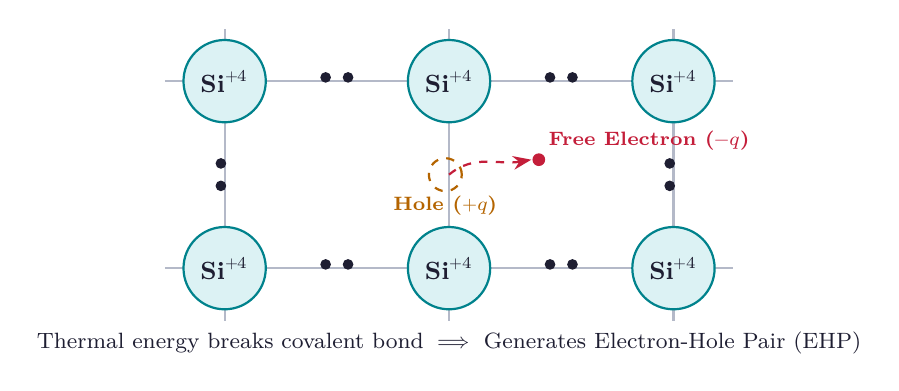
\begin{tikzpicture}[scale=0.95]
  % Define atom coordinates (3x3 grid)
  \foreach \x in {0, 3, 6} {
    \foreach \y in {0, 2.5} {
      \draw[thick, color=mgframe] (\x-0.8, \y) -- (\x+0.8, \y);
      \draw[thick, color=mgframe] (\x, \y-0.7) -- (\x, \y+0.7);
    }
  }
  % Connecting bond lines between atoms
  \draw[thick, color=mgframe] (0.8, 2.5) -- (2.2, 2.5);
  \draw[thick, color=mgframe] (3.8, 2.5) -- (5.2, 2.5);
  \draw[thick, color=mgframe] (0.8, 0) -- (2.2, 0);
  \draw[thick, color=mgframe] (3.8, 0) -- (5.2, 0);
  \draw[thick, color=mgframe] (0, 0.7) -- (0, 1.8);
  \draw[thick, color=mgframe] (3, 0.7) -- (3, 1.8);
  \draw[thick, color=mgframe] (6, 0.7) -- (6, 1.8);

  % Atoms
  \foreach \x in {0, 3, 6} {
    \foreach \y in {0, 2.5} {
      \filldraw[fill=hdrteal, draw=myteal, thick] (\x, \y) circle (0.55) node[font=\small\bfseries\color{mydark}] {$\text{Si}^{+4}$};
    }
  }

  % Valence electron dots (bonded pairs)
  \foreach \x in {1.5, 4.5} {
    \filldraw[color=mydark] (\x-0.15, 2.55) circle (1.8pt);
    \filldraw[color=mydark] (\x+0.15, 2.55) circle (1.8pt);
    \filldraw[color=mydark] (\x-0.15, 0.05) circle (1.8pt);
    \filldraw[color=mydark] (\x+0.15, 0.05) circle (1.8pt);
  }
  \foreach \y in {1.25} {
    \filldraw[color=mydark] (-0.05, \y-0.15) circle (1.8pt);
    \filldraw[color=mydark] (-0.05, \y+0.15) circle (1.8pt);
    \filldraw[color=mydark] (5.95, \y-0.15) circle (1.8pt);
    \filldraw[color=mydark] (5.95, \y+0.15) circle (1.8pt);
  }

  % Broken bond at center vertical bridge
  \draw[dashed, thick, color=myamber] (2.95, 1.25) circle (0.22) node[below=4pt, font=\scriptsize\bfseries\color{myamber}] {Hole ($+q$)};
  \filldraw[color=myred] (4.2, 1.45) circle (2.2pt) node[above right, font=\scriptsize\bfseries\color{myred}] {Free Electron ($-q$)};
  \draw[-Stealth, thick, dashed, color=myred] (3.0, 1.25) to[out=40, in=190] (4.1, 1.45);
  \node[font=\footnotesize\color{mydark}, align=center] at (3, -1.0) {Thermal energy breaks covalent bond $\implies$ Generates Electron-Hole Pair (EHP)};
\end{tikzpicture}
\end{tcolorbox}

\subsection{The Concept of Holes and Hole Conduction}
A \textbf{hole} is a conceptual quasiparticle representing an unoccupied quantum electronic state (vacancy) in an otherwise nearly filled valence band.

\begin{tcolorbox}[defbox, title={\textbf{Physics and Fundamental Properties of Holes}}]
\begin{itemize}[leftmargin=*, itemsep=3pt]
  \item \textbf{Effective Positive Charge ($+q$):} The absence of an electron (charge $-q$) from a neutral atom vacancy within a crystal lattice results in a net local positive charge of $+q = +1.602 \times 10^{-19}\,\text{C}$.
  \item \textbf{Mechanism of Hole Conduction:} When an electric field $\vec{\mathcal{E}}$ is applied across a semiconductor, an electron from an adjacent covalent bond hops into the vacancy in the direction opposite to $\vec{\mathcal{E}}$. This creates a new vacancy at the adjacent site. Macroscopically, this sequential valence electron hopping appears as the directed physical motion of a \textbf{positive charge carrier} (hole) traveling in the direction of the applied electric field $\vec{\mathcal{E}}$.
  \item \textbf{Positive Effective Mass ($m_h^*$):} Near the top of the valence band, the $E\text{-}k$ energy-momentum dispersion has downward curvature ($\frac{d^2 E}{dk^2} < 0$). An electron missing from a negative-curvature state behaves dynamically under external forces as a particle with a \textbf{positive effective mass}:
  \begin{equation}
    m_h^* = -\frac{\hbar^2}{\left(\frac{d^2 E}{dk^2}\right)_{\text{VB max}}} > 0
  \end{equation}
  \item \textbf{Hole Mobility Comparison ($\mu_p < \mu_n$):} Hole transport requires overcoming local covalent bonding potentials and hopping across tightly bound valence orbitals, experiencing higher acoustic phonon scattering. Consequently, hole mobility is always substantially lower than conduction-band electron mobility (in Silicon at $300\,\text{K}$, $\mu_n \approx 1350\,\text{cm}^2/\text{V}\cdot\text{s}$ while $\mu_p \approx 480\,\text{cm}^2/\text{V}\cdot\text{s}$).
\end{itemize}
\end{tcolorbox}

% ===============================================================================
\section{Energy Band Theory in Crystals}
% ===============================================================================

\subsection{Formation of Energy Bands}
In an isolated atom, electrons occupy sharp, discrete quantum energy levels ($1s, 2s, 2p, 3s, 3p, \dots$) governed by the Schr\"{o}dinger equation. When $N$ atoms are brought together to form a crystal lattice:

\begin{enumerate}[label=\arabic*., leftmargin=*]
  \item As interatomic spacing decreases, the wavefunctions of outermost valence electrons begin to overlap.
  \item By the \textbf{Pauli Exclusion Principle}, no two electrons in the interacting system can occupy the exact same quantum state.
  \item Each discrete atomic energy level splits into $N$ distinct, extremely closely spaced sub-levels. Because $N \sim 10^{22}\,\text{cm}^{-3}$ in a typical solid, these split levels merge into continuous \textbf{energy bands}.
  \item The energy gaps between allowed bands where no valid electron quantum states can exist are called \textbf{forbidden energy gaps} or \textbf{bandgaps} ($E_g$).
\end{enumerate}

\begin{tcolorbox}[defbox, title={\textbf{Energy Band Definitions}}]
\begin{itemize}[leftmargin=*, itemsep=2pt, topsep=0pt]
  \item \textbf{Valence Band (VB):} The highest occupied energy band formed by valence electrons. At $0\,\text{K}$, it is completely filled.
  \item \textbf{Conduction Band (CB):} The lowest unoccupied or partially filled energy band where free electrons participate in electrical conduction.
  \item \textbf{Forbidden Bandgap ($E_g$):} The energy difference between the conduction band minimum ($E_c$) and valence band maximum ($E_v$): $E_g = E_c - E_v$.
\end{itemize}
\end{tcolorbox}

\subsection{Direct vs. Indirect Bandgap Semiconductors}
The relationship between electron energy $E$ and crystal wavevector (momentum) $k$ is given by the $E$-$k$ dispersion diagram:

\begin{itemize}[leftmargin=*, itemsep=3.5pt]
  \item \textbf{Direct Bandgap Semiconductor:} The conduction band minimum and valence band maximum occur at the \textbf{same wavevector} ($k = 0$). An electron recombining with a hole across $E_g$ releases energy directly as a photon ($\Delta k = 0$):
  \begin{equation}
    E_g = h\nu = \frac{hc}{\lambda}
  \end{equation}
  \textbf{Examples:} Gallium Arsenide ($\text{GaAs}$, $E_g = 1.42\,\text{eV}$), Indium Phosphide ($\text{InP}$). Used in LEDs, laser diodes, and photodetectors.
  \item \textbf{Indirect Bandgap Semiconductor:} The conduction band minimum occurs at a \textbf{different wavevector} ($k \neq 0$) than the valence band maximum ($k = 0$). Recombination requires both an energy change and a crystal momentum change, necessitating the emission or absorption of a lattice vibration or \textbf{phonon}:
  \begin{equation}
    \Delta E = h\nu \pm E_{\text{phonon}}, \quad \Delta k = k_{\text{phonon}}
  \end{equation}
  Because a three-particle interaction (electron, hole, phonon) has low transition probability, nonradiative recombination dominates.
  \textbf{Examples:} Silicon ($\text{Si}$, $E_g = 1.12\,\text{eV}$), Germanium ($\text{Ge}$, $E_g = 0.66\,\text{eV}$). Unsuitable for efficient light emitters.
\end{itemize}

\begin{tcolorbox}[tikzbox, title={Direct vs. Indirect Bandgap Transitions ($E$-$k$ Diagrams)}]
\centering
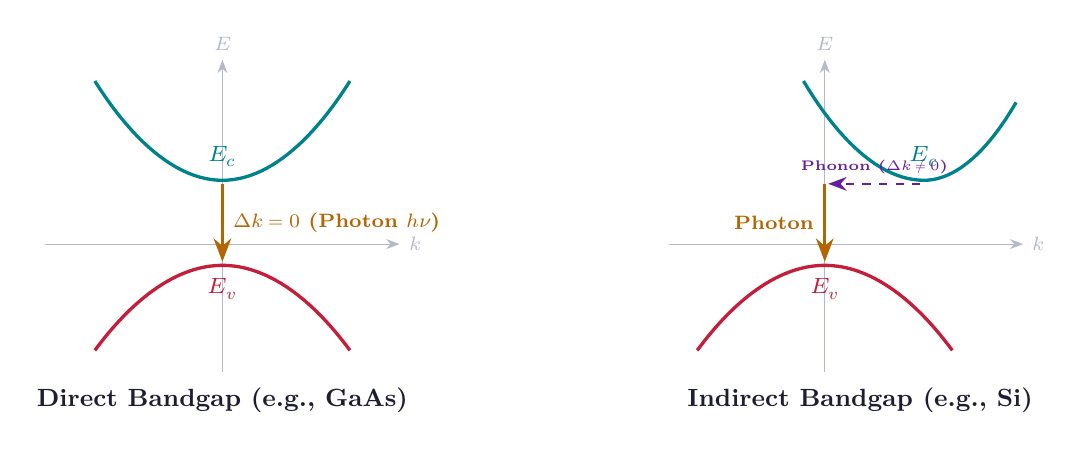
\begin{tikzpicture}[scale=0.9]
  % Direct Bandgap (Left)
  \begin{scope}[xshift=-4.5cm]
    \draw[-Stealth, color=mgframe] (-2.5,0) -- (2.5,0) node[right, font=\scriptsize] {$k$};
    \draw[-Stealth, color=mgframe] (0,-1.8) -- (0,2.6) node[above, font=\scriptsize] {$E$};
    % Conduction Band parabola
    \draw[very thick, color=myteal] (-1.8, 2.3) parabola bend (0, 0.9) (1.8, 2.3);
    \node[above, font=\footnotesize\bfseries\color{myteal}] at (0, 0.95) {$E_c$};
    % Valence Band parabola
    \draw[very thick, color=myred] (-1.8, -1.5) parabola bend (0, -0.3) (1.8, -1.5);
    \node[below, font=\footnotesize\bfseries\color{myred}] at (0, -0.35) {$E_v$};
    % Direct vertical transition
    \draw[-Stealth, very thick, color=myamber] (0, 0.85) -- (0, -0.25) node[midway, right, font=\scriptsize\bfseries\color{myamber}] {$\Delta k = 0$ (Photon $h\nu$)};
    \node[font=\small\bfseries\color{mydark}] at (0, -2.2) {Direct Bandgap (e.g., GaAs)};
  \end{scope}

  % Indirect Bandgap (Right)
  \begin{scope}[xshift=4.0cm]
    \draw[-Stealth, color=mgframe] (-2.2,0) -- (2.8,0) node[right, font=\scriptsize] {$k$};
    \draw[-Stealth, color=mgframe] (0,-1.8) -- (0,2.6) node[above, font=\scriptsize] {$E$};
    % Conduction Band parabola (shifted minimum)
    \draw[very thick, color=myteal] (-0.3, 2.3) parabola bend (1.4, 0.9) (2.7, 2.0);
    \node[above, font=\footnotesize\bfseries\color{myteal}] at (1.4, 0.95) {$E_c$};
    % Valence Band parabola (centered at k=0)
    \draw[very thick, color=myred] (-1.8, -1.5) parabola bend (0, -0.3) (1.8, -1.5);
    \node[below, font=\footnotesize\bfseries\color{myred}] at (0, -0.35) {$E_v$};
    % Two-step transition (phonon + photon)
    \draw[-Stealth, thick, dashed, color=mypurple] (1.35, 0.85) -- (0.05, 0.85) node[midway, above, font=\tiny\bfseries\color{mypurple}] {Phonon ($\Delta k \neq 0$)};
    \draw[-Stealth, very thick, color=myamber] (0, 0.85) -- (0, -0.25) node[midway, left, font=\scriptsize\bfseries\color{myamber}] {Photon};
    \node[font=\small\bfseries\color{mydark}] at (0.5, -2.2) {Indirect Bandgap (e.g., Si)};
  \end{scope}
\end{tikzpicture}
\end{tcolorbox}

% ===============================================================================
\section{Classification: Metals, Semiconductors, and Insulators}
% ===============================================================================

Solids are classified into three categories based on the magnitude of their forbidden energy gap ($E_g$) and their room-temperature electrical conductivity:

\par\vspace{6pt}\noindent
\begingroup
\setlength{\tabcolsep}{3.5pt}
\setlength{\extrarowheight}{3pt}
\renewcommand{\arraystretch}{1.35}
\begin{tabularx}{\linewidth}{|B{2.4cm}|Y|Y|Y|}
\hline
\textbf{Parameter} & \textbf{Insulator} & \textbf{Semiconductor} & \textbf{Metal (Conductor)} \\
\hline
Forbidden Gap ($E_g$) & Very large ($E_g > 3\,\text{eV}$ to $6\,\text{eV}$) & Moderate ($0.6\,\text{eV} \le E_g \le 2.0\,\text{eV}$) & Zero ($E_g = 0\,\text{eV}$, bands overlap) \\
\hline
Conduction Band at $0\,\text{K}$ & Completely empty & Completely empty & Partially filled or overlaps VB \\
\hline
Conductivity ($\sigma$) & Extremely low ($< 10^{-10}\,\text{S/cm}$) & Intermediate ($10^{-6}$ to $10^{2}\,\text{S/cm}$) & Extremely high ($10^{4}$ to $10^{6}\,\text{S/cm}$) \\
\hline
Temperature Coefficient of Resistance & Negative ($\text{NTC}$): Resistance decreases as $T$ increases & Negative ($\text{NTC}$): $R$ decreases exponentially as $T$ rises & Positive ($\text{PTC}$): Resistance increases due to phonon scattering \\
\hline
Typical Materials & Diamond ($5.5\,\text{eV}$), $\text{SiO}_2$ ($9\,\text{eV}$) & $\text{Si}$ ($1.12\,\text{eV}$), $\text{Ge}$ ($0.66\,\text{eV}$), $\text{GaAs}$ & Copper ($\text{Cu}$), Aluminum ($\text{Al}$), Gold \\
\hline
\end{tabularx}
\endgroup

\subsection{Temperature Dependence of Bandgap Energy}
The bandgap of a semiconductor decreases slightly as temperature increases due to thermal lattice expansion and increased electron-phonon interaction. Varshni's empirical formula models this variation:

\begin{equation}
  E_g(T) = E_g(0) - \frac{\alpha T^2}{T + \beta}
\end{equation}

For Silicon: $E_g(0) = 1.17\,\text{eV}$, $\alpha = 4.73 \times 10^{-4}\,\text{eV/K}$, $\beta = 636\,\text{K}$. At $300\,\text{K}$, $E_g \approx 1.12\,\text{eV}$.

% ===============================================================================
\section{Fermi Level and Carrier Statistics}
% ===============================================================================

\subsection{Fermi-Dirac Distribution Function}
Electrons are fermions (spin-$1/2$ particles) subject to the Pauli exclusion principle. The probability $f(E)$ that an available quantum energy state $E$ is occupied by an electron at thermodynamic equilibrium temperature $T$ is governed by the \textbf{Fermi-Dirac distribution}:

\begin{equation}
  f(E) = \frac{1}{1 + \exp\left(\displaystyle\frac{E - E_F}{k T}\right)}
\end{equation}

where $k = 8.617 \times 10^{-5}\,\text{eV/K} = 1.38 \times 10^{-23}\,\text{J/K}$ is Boltzmann's constant, and $E_F$ is the \textbf{Fermi energy level}.

\begin{tcolorbox}[defbox, title={\textbf{Physical Meaning and Properties of Fermi Level $E_F$}}]
\begin{itemize}[leftmargin=*, itemsep=3pt, topsep=0pt]
  \item At absolute zero ($T = 0\,\text{K}$):
    \begin{equation}
      f(E) = 
      \begin{cases} 
        1, & E < E_F \quad \text{(all states below $E_F$ are completely filled)} \\ 
        0, & E > E_F \quad \text{(all states above $E_F$ are completely empty)} 
      \end{cases}
    \end{equation}
    $E_F$ is the highest filled energy level at absolute zero temperature.
  \item At any finite temperature ($T > 0\,\text{K}$):
    When $E = E_F$, the exponential argument vanishes:
    \begin{equation}
      f(E_F) = \frac{1}{1 + e^0} = \frac{1}{2} = 0.5
    \end{equation}
    The Fermi level is the energy state having a $50\%$ probability of being occupied by an electron.
  \item The probability of a state at $E$ being empty (occupied by a hole) is:
    \begin{equation}
      1 - f(E) = \frac{1}{1 + \exp\left(\displaystyle\frac{E_F - E}{k T}\right)}
    \end{equation}
\end{itemize}
\end{tcolorbox}

\begin{tcolorbox}[tikzbox, title={Fermi-Dirac Distribution at Different Temperatures}]
\centering
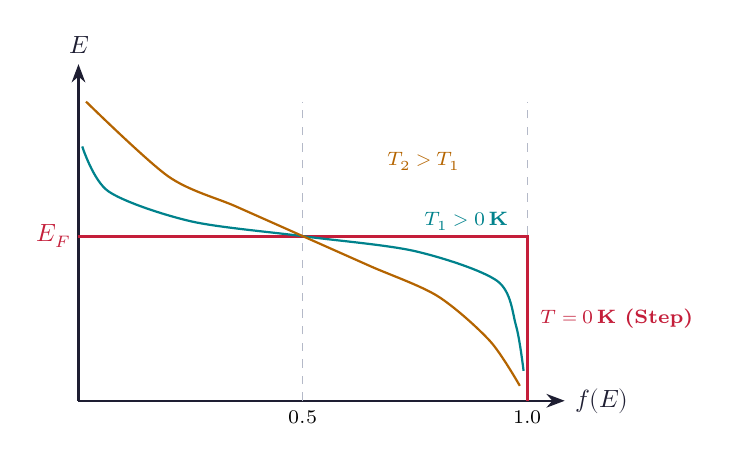
\begin{tikzpicture}[scale=0.95]
  \draw[-Stealth, thick, color=mydark] (0,0) -- (6.5,0) node[right, font=\small] {$f(E)$};
  \draw[-Stealth, thick, color=mydark] (0,0) -- (0,4.5) node[above, font=\small] {$E$};

  % Coordinates
  \coordinate (O) at (0,0);
  \coordinate (fhalf) at (3.0, 2.2);
  \coordinate (EF) at (0, 2.2);
  \coordinate (f1) at (6.0, 0);

  % Axis ticks and labels
  \draw[dashed, color=mgframe] (3.0, 0) -- (3.0, 4.0);
  \node[below, font=\scriptsize] at (3.0, 0) {$0.5$};
  \draw[dashed, color=mgframe] (6.0, 0) -- (6.0, 4.0);
  \node[below, font=\scriptsize] at (6.0, 0) {$1.0$};
  \node[left, font=\small\bfseries\color{myred}] at (0, 2.2) {$E_F$};

  % T = 0 K step function
  \draw[very thick, color=myred] (6.0, 0) -- (6.0, 2.2) -- (0, 2.2);
  \node[right, font=\scriptsize\bfseries\color{myred}] at (6.05, 1.1) {$T = 0\,\text{K}$ (Step)};

  % T1 > 0 K curve
  \draw[thick, color=myteal, smooth] plot coordinates {
    (5.95, 0.4) (5.85, 1.0) (5.6, 1.6) (4.5, 2.0) (3.0, 2.2) (1.5, 2.4) (0.4, 2.8) (0.05, 3.4)
  };
  \node[right, font=\scriptsize\bfseries\color{myteal}] at (4.5, 2.4) {$T_1 > 0\,\text{K}$};

  % T2 > T1 curve
  \draw[thick, color=myamber, smooth] plot coordinates {
    (5.9, 0.2) (5.5, 0.8) (4.8, 1.4) (3.9, 1.8) (3.0, 2.2) (2.1, 2.6) (1.2, 3.0) (0.1, 4.0)
  };
  \node[right, font=\scriptsize\bfseries\color{myamber}] at (4.0, 3.2) {$T_2 > T_1$};
\end{tikzpicture}
\end{tcolorbox}

% ===============================================================================
\section{Intrinsic and Extrinsic Semiconductors}
% ===============================================================================

\subsection{Intrinsic Semiconductors and Intrinsic Carrier Concentration}
An \textbf{intrinsic semiconductor} is a chemically pure semiconductor crystal containing no significant impurities or structural lattice defects.

\begin{itemize}[leftmargin=*, itemsep=3pt]
  \item Free carriers are generated purely by thermal breakage of covalent bonds.
  \item Every electron elevated to the conduction band leaves behind exactly one vacant state (hole) in the valence band:
  \begin{equation}
    n = p = n_i
  \end{equation}
  where $n$ is electron concentration ($\text{cm}^{-3}$), $p$ is hole concentration ($\text{cm}^{-3}$), and $n_i$ is the \textbf{intrinsic carrier concentration}.
  \item For Silicon at $300\,\text{K}$, $n_i \approx 1.5 \times 10^{10}\,\text{cm}^{-3}$. For Germanium, $n_i \approx 2.4 \times 10^{13}\,\text{cm}^{-3}$. For GaAs, $n_i \approx 1.8 \times 10^6\,\text{cm}^{-3}$.
\end{itemize}

\subsection{Effective Density of States and Equilibrium Carrier Concentrations}
Integrating the product of the density of available quantum states $g(E)$ and the Fermi-Dirac distribution $f(E)$ under the Maxwell-Boltzmann approximation ($E - E_F \gg 3kT$) yields:

\begin{tcolorbox}[formulabox, title={\textbf{Equilibrium Carrier Concentrations and Effective Densities of States}}]
\begin{align}
  n_0 &= N_c \exp\left(-\frac{E_c - E_F}{k T}\right) \\
  p_0 &= N_v \exp\left(-\frac{E_F - E_v}{k T}\right)
\end{align}
where $N_c$ and $N_v$ are the \textbf{effective densities of states} in the conduction and valence bands:
\begin{equation}
  N_c = 2\left(\frac{2\pi m_e^* k T}{h^2}\right)^{3/2}, \qquad N_v = 2\left(\frac{2\pi m_h^* k T}{h^2}\right)^{3/2}
\end{equation}
where $m_e^*$ and $m_h^*$ are the density-of-states effective masses for electrons and holes. For Silicon at $300\,\text{K}$, $N_c \approx 2.8 \times 10^{19}\,\text{cm}^{-3}$ and $N_v \approx 1.04 \times 10^{19}\,\text{cm}^{-3}$.
\end{tcolorbox}

\subsection{The Law of Mass Action}
Multiplying the equilibrium electron concentration $n_0$ and hole concentration $p_0$:

\begin{equation}
  n_0 p_0 = N_c N_v \exp\left(-\frac{E_c - E_F + E_F - E_v}{k T}\right) = N_c N_v \exp\left(-\frac{E_g}{k T}\right)
\end{equation}

Because the product is completely independent of the Fermi level $E_F$ and doping concentrations:

\begin{tcolorbox}[formulabox, title={\textbf{Law of Mass Action}}]
Under thermal equilibrium conditions, for any semiconductor (intrinsic or extrinsic):
\begin{equation}
  n_0 p_0 = n_i^2 = N_c N_v \exp\left(-\frac{E_g}{k T}\right)
\end{equation}
The intrinsic carrier concentration depends exponentially on temperature and bandgap:
\begin{equation}
  n_i = \sqrt{N_c N_v}\,\exp\left(-\frac{E_g}{2 k T}\right) \propto T^{3/2} \exp\left(-\frac{E_g}{2 k T}\right)
\end{equation}
\end{tcolorbox}

\subsection{Position of the Intrinsic Fermi Level (\texorpdfstring{$E_i$}{Ei})}
In an intrinsic semiconductor, $n_0 = p_0 = n_i$. Equating $n_0$ and $p_0$:

\begin{align*}
  N_c \exp\left(-\frac{E_c - E_i}{k T}\right) &= N_v \exp\left(-\frac{E_i - E_v}{k T}\right) \\
  \exp\left(\frac{2E_i - (E_c + E_v)}{k T}\right) &= \frac{N_v}{N_c} = \left(\frac{m_h^*}{m_e^*}\right)^{3/2}
\end{align*}

Solving for $E_i$:
\begin{equation}
  E_i = \frac{E_c + E_v}{2} + \frac{3}{4} k T \ln\left(\frac{m_h^*}{m_e^*}\right)
\end{equation}

\textbf{Key Takeaway:} At $T = 0\,\text{K}$, or if $m_e^* = m_h^*$, $E_i$ lies precisely at the midgap: $E_{\text{midgap}} = (E_c + E_v)/2$. Because $m_h^* > m_e^*$ in Silicon, $E_i$ lies slightly above midgap by a few millielectronvolts at $300\,\text{K}$.

\subsection{Extrinsic Semiconductors: n-type and p-type Doping}
Doping is the intentional introduction of specific trace impurity atoms into an intrinsic semiconductor to selectively increase either electron or hole concentration.

\begin{itemize}[leftmargin=*, itemsep=3.5pt]
  \item \textbf{n-type Doping (Donor Impurities):} Pentavalent atoms (Group V: Phosphorus $\text{P}$, Arsenic $\text{As}$, Antimony $\text{Sb}$) replace Silicon atoms. Four valence electrons form covalent bonds, while the fifth weakly bound electron occupies a discrete energy level $E_d$ located very close to the conduction band ($E_c - E_d \approx 0.045\,\text{eV}$ in $\text{Si}$). At room temperature, all donor atoms ionize:
  \begin{equation}
    n_0 \approx N_D, \qquad p_0 = \frac{n_i^2}{N_D} \ll n_0
  \end{equation}
  The Fermi level shifts upward toward the conduction band:
  \begin{equation}
    E_F - E_i = k T \ln\left(\frac{N_D}{n_i}\right) \implies E_c - E_F = k T \ln\left(\frac{N_c}{N_D}\right)
  \end{equation}

  \item \textbf{p-type Doping (Acceptor Impurities):} Trivalent atoms (Group III: Boron $\text{B}$, Gallium $\text{Ga}$, Indium $\text{In}$) replace Silicon atoms. Three valence electrons form bonds, leaving an empty bond that readily accepts an electron from the valence band, creating a mobile hole. The acceptor energy level $E_a$ lies just above the valence band ($E_a - E_v \approx 0.045\,\text{eV}$ in $\text{Si}$). At room temperature:
  \begin{equation}
    p_0 \approx N_A, \qquad n_0 = \frac{n_i^2}{N_A} \ll p_0
  \end{equation}
  The Fermi level shifts downward toward the valence band:
  \begin{equation}
    E_i - E_F = k T \ln\left(\frac{N_A}{n_i}\right) \implies E_F - E_v = k T \ln\left(\frac{N_v}{N_A}\right)
  \end{equation}
\end{itemize}

\begin{tcolorbox}[tikzbox, title={Energy Band Diagrams for Intrinsic, n-type, and p-type Semiconductors}]
\centering
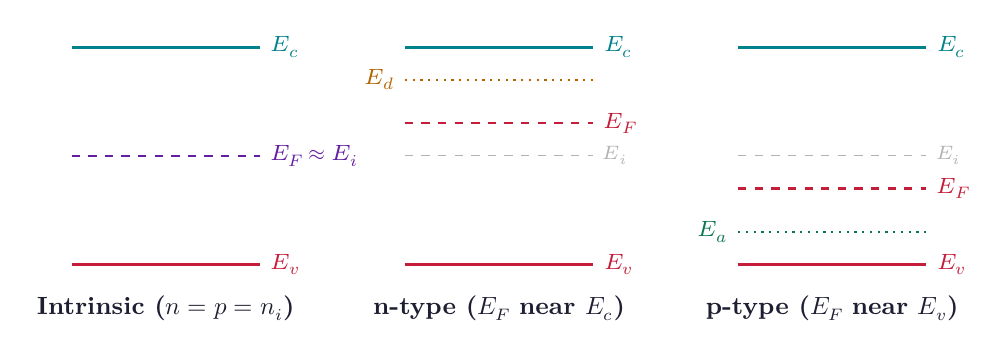
\begin{tikzpicture}[scale=0.92]
  % Intrinsic (Left)
  \begin{scope}[xshift=-4.6cm]
    \draw[very thick, color=myteal] (0, 3.3) -- (2.6, 3.3) node[right, font=\footnotesize\bfseries\color{myteal}] {$E_c$};
    \draw[dashed, thick, color=mypurple] (0, 1.8) -- (2.6, 1.8) node[right, font=\footnotesize\bfseries\color{mypurple}] {$E_F \approx E_i$};
    \draw[very thick, color=myred] (0, 0.3) -- (2.6, 0.3) node[right, font=\footnotesize\bfseries\color{myred}] {$E_v$};
    \node[font=\small\bfseries\color{mydark}] at (1.3, -0.3) {Intrinsic ($n=p=n_i$)};
  \end{scope}

  % n-type (Center)
  \begin{scope}[xshift=0cm]
    \draw[very thick, color=myteal] (0, 3.3) -- (2.6, 3.3) node[right, font=\footnotesize\bfseries\color{myteal}] {$E_c$};
    \draw[dotted, thick, color=myamber] (0, 2.85) node[left, font=\footnotesize\bfseries\color{myamber}] {$E_d$} -- (2.6, 2.85);
    \draw[dashed, thick, color=myred] (0, 2.25) -- (2.6, 2.25) node[right, font=\footnotesize\bfseries\color{myred}] {$E_F$};
    \draw[dashed, thin, color=gray!60] (0, 1.8) -- (2.6, 1.8) node[right, font=\scriptsize\color{gray}] {$E_i$};
    \draw[very thick, color=myred] (0, 0.3) -- (2.6, 0.3) node[right, font=\footnotesize\bfseries\color{myred}] {$E_v$};
    \node[font=\small\bfseries\color{mydark}] at (1.3, -0.3) {n-type ($E_F$ near $E_c$)};
  \end{scope}

  % p-type (Right)
  \begin{scope}[xshift=4.6cm]
    \draw[very thick, color=myteal] (0, 3.3) -- (2.6, 3.3) node[right, font=\footnotesize\bfseries\color{myteal}] {$E_c$};
    \draw[dashed, thin, color=gray!60] (0, 1.8) -- (2.6, 1.8) node[right, font=\scriptsize\color{gray}] {$E_i$};
    \draw[dashed, thick, color=myred] (0, 1.35) -- (2.6, 1.35) node[right, font=\footnotesize\bfseries\color{myred}] {$E_F$};
    \draw[dotted, thick, color=mygreen] (0, 0.75) node[left, font=\footnotesize\bfseries\color{mygreen}] {$E_a$} -- (2.6, 0.75);
    \draw[very thick, color=myred] (0, 0.3) -- (2.6, 0.3) node[right, font=\footnotesize\bfseries\color{myred}] {$E_v$};
    \node[font=\small\bfseries\color{mydark}] at (1.3, -0.3) {p-type ($E_F$ near $E_v$)};
  \end{scope}
\end{tikzpicture}
\end{tcolorbox}

\subsection{Temperature Dependence of Extrinsic Carrier Concentration}
In an n-type semiconductor ($N_D \gg n_i$), electron concentration varies across three distinct temperature regimes:

\begin{enumerate}[label=\arabic*., leftmargin=*]
  \item \textbf{Ionization (Freeze-out) Regime ($T < 100\,\text{K}$):} Thermal energy is insufficient to ionize all donor electrons. As temperature rises, electrons transition from $E_d$ to $E_c$. Carrier concentration increases rapidly: $n_0 \propto \exp(-\Delta E_d / 2kT)$.
  \item \textbf{Extrinsic (Exhaustion / Saturation) Regime ($100\,\text{K} \le T \le 450\,\text{K}$):} All donor impurities are fully ionized, while intrinsic generation across $E_g$ remains negligible ($n_i \ll N_D$). Carrier concentration remains flat and constant: $n_0 \approx N_D$. This is the standard operational regime for electronic devices.
  \item \textbf{Intrinsic Regime ($T > 450\,\text{K}$):} Thermally generated intrinsic carriers across the bandgap exceed the donor concentration ($n_i \gg N_D$). The semiconductor loses its extrinsic properties and behaves as an intrinsic material ($n_0 \approx n_i \propto T^{3/2} e^{-E_g/2kT}$).
\end{enumerate}

% ===============================================================================
\section{Carrier Transport: Drift and Diffusion}
% ===============================================================================

Charge carriers in semiconductors move under the influence of two primary driving forces: electric fields (\textbf{drift}) and carrier concentration gradients (\textbf{diffusion}).

\subsection{Carrier Drift and Mobility}
When an electric field $\mathcal{E}$ is applied across a semiconductor, electrons and holes accelerate until they collide with the vibrating lattice atoms (phonons) or ionized impurity atoms. The net average velocity acquired between collisions is the \textbf{drift velocity} ($v_d$):

\begin{equation}
  v_{d,n} = -\mu_n \mathcal{E}, \qquad v_{d,p} = \mu_p \mathcal{E}
\end{equation}

where $\mu_n$ and $\mu_p$ are the electron and hole \textbf{carrier mobilities} ($\text{cm}^2/\text{V}\cdot\text{s}$):

\begin{equation}
  \mu = \frac{q \tau_c}{m^*}
\end{equation}

where $\tau_c$ is the mean free collision time, and $m^*$ is the conductivity effective mass. Because $m_e^* < m_h^*$ in Silicon, $\mu_n \approx 1350\,\text{cm}^2/\text{V}\cdot\text{s}$ is significantly higher than $\mu_p \approx 480\,\text{cm}^2/\text{V}\cdot\text{s}$.

\subsubsection{Scattering Mechanisms and Temperature Dependence}
By \textbf{Matthiessen's Rule}, the total effective mobility $\mu$ is limited by the reciprocal sum of independent scattering processes:

\begin{equation}
  \frac{1}{\mu} = \frac{1}{\mu_{\text{lattice}}} + \frac{1}{\mu_{\text{impurity}}}
\end{equation}

\begin{itemize}[leftmargin=*, itemsep=3pt]
  \item \textbf{Lattice (Acoustic Phonon) Scattering:} Thermal vibrations of lattice atoms scatter carriers. As temperature increases, lattice vibrations intensify: $\mu_{\text{lattice}} \propto T^{-3/2}$.
  \item \textbf{Ionized Impurity Scattering:} Electrostatic Coulomb deflection of carriers as they travel past ionized donor ($N_D^+$) or acceptor ($N_A^-$) impurities. At higher temperatures, thermal velocity increases, carriers spend less time near impurity ions, and scattering diminishes: $\mu_{\text{impurity}} \propto T^{3/2} / N_I$.
\end{itemize}

\subsection{Drift Current Density and Conductivity}
The current density due to drift of electrons and holes under electric field $\mathcal{E}$ is:

\begin{equation}
  J_{\text{drift}} = J_{n,\text{drift}} + J_{p,\text{drift}} = q n \mu_n \mathcal{E} + q p \mu_p \mathcal{E} = \sigma \mathcal{E}
\end{equation}

where the \textbf{electrical conductivity} $\sigma$ and resistivity $\rho$ are:

\begin{tcolorbox}[formulabox, title={\textbf{Conductivity and Resistivity}}]
\begin{align}
  \sigma &= q (n \mu_n + p \mu_p) \quad (\text{S/cm}) \\
  \rho &= \frac{1}{\sigma} = \frac{1}{q (n \mu_n + p \mu_p)} \quad (\Omega\cdot\text{cm})
\end{align}
For an n-type semiconductor ($n \approx N_D \gg p$): $\sigma \approx q N_D \mu_n$.
\end{tcolorbox}

\subsection{Carrier Diffusion}
Carrier diffusion is the net movement of charge carriers from a region of higher concentration to a region of lower concentration due to random thermal Brownian motion. By Fick's first law of diffusion:

\begin{tcolorbox}[formulabox, title={\textbf{Diffusion Current Densities}}]
\begin{align}
  J_{n,\text{diff}} &= +q D_n \frac{dn}{dx} \\
  J_{p,\text{diff}} &= -q D_p \frac{dp}{dx}
\end{align}
where $D_n$ and $D_p$ are the \textbf{diffusion coefficients} ($\text{cm}^2/\text{s}$). The negative sign in $J_{p,\text{diff}}$ arises because holes diffuse down the concentration gradient ($\nabla p < 0$), carrying positive charge in the direction of diffusion. Electrons carry negative charge, producing a positive sign.
\end{tcolorbox}

\subsection{Total Current Density}
Combining drift and diffusion components yields the complete one-dimensional current equations:

\begin{equation}
  J_n = J_{n,\text{drift}} + J_{n,\text{diff}} = q n \mu_n \mathcal{E} + q D_n \frac{dn}{dx}
\end{equation}
\begin{equation}
  J_p = J_{p,\text{drift}} + J_{p,\text{diff}} = q p \mu_p \mathcal{E} - q D_p \frac{dp}{dx}
\end{equation}
\begin{equation}
  J_{\text{total}} = J_n + J_p
\end{equation}

\subsection{The Einstein Relation}
Under thermodynamic equilibrium, no external current can flow ($J_n = 0, J_p = 0$). Setting $J_p = 0$ in a non-uniformly doped semiconductor where a built-in internal electric field balances carrier diffusion:

\begin{align*}
  q p \mu_p \mathcal{E} &= q D_p \frac{dp}{dx} \\
  \mathcal{E} &= \frac{D_p}{\mu_p} \frac{1}{p} \frac{dp}{dx}
\end{align*}

Using the electrostatic potential $\mathcal{E} = -\frac{dV}{dx}$ and Boltzmann relationship $p(x) = n_i \exp\left(\frac{E_i - E_F}{kT}\right) = n_i \exp\left(-\frac{qV}{kT}\right)$, we find $\frac{1}{p}\frac{dp}{dx} = -\frac{q}{kT}\frac{dV}{dx} = \frac{q}{kT}\mathcal{E}$. Substituting yields:

\begin{tcolorbox}[formulabox, title={\textbf{Einstein Relation}}]
\begin{equation}
  \frac{D_n}{\mu_n} = \frac{D_p}{\mu_p} = \frac{k T}{q} = V_T
\end{equation}
where $V_T = \frac{kT}{q} \approx 25.9\,\text{mV}$ at $T = 300\,\text{K}$ is the \textbf{thermal voltage}.
\end{tcolorbox}

% ===============================================================================
\section{Generation, Recombination, and Minority Carrier Injection}
% ===============================================================================

\subsection{Carrier Generation and Recombination Mechanisms}
\begin{itemize}[leftmargin=*, itemsep=3pt]
  \item \textbf{Generation ($G$):} The process whereby electron-hole pairs are created. Mechanisms include thermal generation ($G_{\text{th}}$) and optical absorption ($G_L$).
  \item \textbf{Recombination ($R$):} The process whereby an electron drops into a vacant hole state, annihilating both carriers and releasing energy.
\end{itemize}

The three principal physical mechanisms of recombination are:
\begin{enumerate}[label=\arabic*., leftmargin=*]
  \item \textbf{Direct Band-to-Band Recombination:} An electron transitions directly from the CB to VB, emitting a photon. Dominates in direct bandgap materials ($\text{GaAs}$). Recombination rate $R \propto n \cdot p$.
  \item \textbf{Shockley-Read-Hall (SRH) Recombination:} Mediated by deep localized energy states or ``traps'' located near the center of the bandgap created by crystal defects or metallic impurities (Gold, Platinum). Dominates in indirect bandgap semiconductors ($\text{Si}, \text{Ge}$).
  \item \textbf{Auger Recombination:} The energy released when an electron recombines with a hole is transferred to a third carrier (electron or hole), kicking it higher into its band. Important under very high injection levels and heavily doped regions.
\end{enumerate}

\subsection{Excess Carriers and Low-Level Injection}
When excess carriers are introduced into a semiconductor (via illumination or forward-biased p-n junction injection):
\begin{equation}
  n(t) = n_0 + \Delta n(t), \qquad p(t) = p_0 + \Delta p(t)
\end{equation}
where $n_0, p_0$ are equilibrium concentrations, and $\Delta n, \Delta p$ are excess carrier concentrations. In non-breakdown conditions, $\Delta n = \Delta p$.

\begin{tcolorbox}[defbox, title={\textbf{Low-Level Injection Condition}}]
Low-level injection occurs when the excess carrier density is much smaller than the thermal equilibrium majority carrier density:
\begin{itemize}[leftmargin=*, itemsep=2pt, topsep=0pt]
  \item For n-type: $\Delta p = \Delta n \ll n_0 \implies n \approx n_0$, but $p = p_0 + \Delta p \gg p_0$.
  \item For p-type: $\Delta n = \Delta p \ll p_0 \implies p \approx p_0$, but $n = n_0 + \Delta n \gg n_0$.
\end{itemize}
Under low-level injection, majority carrier concentration remains virtually unchanged, but minority carrier concentration changes by orders of magnitude.
\end{tcolorbox}

\subsection{Minority Carrier Lifetime and Diffusion Length}
The net rate of recombination of excess minority holes in an n-type material is proportional to the excess density:
\begin{equation}
  R - G_{\text{th}} = \frac{\Delta p}{\tau_p}
\end{equation}
where $\tau_p$ is the \textbf{minority carrier lifetime}. When excess carrier generation ceases at $t=0$, the excess carriers decay exponentially:
\begin{equation}
  \Delta p(t) = \Delta p(0) \exp\left(-\frac{t}{\tau_p}\right)
\end{equation}

During its lifetime $\tau_p$, an excess carrier diffuses an average distance called the \textbf{minority carrier diffusion length} ($L$):

\begin{tcolorbox}[formulabox, title={\textbf{Diffusion Lengths}}]
\begin{equation}
  L_p = \sqrt{D_p \tau_p}, \qquad L_n = \sqrt{D_n \tau_n}
\end{equation}
\end{tcolorbox}

% ===============================================================================
\section{Poisson's Equation and the Continuity Equation}
% ===============================================================================

\subsection{Poisson's Equation}
Poisson's equation relates the spatial distribution of electrostatic potential $V(x)$ and electric field $\mathcal{E}(x)$ to the net volume charge density $\rho(x)$ using Gauss's law ($\nabla \cdot \vec{\mathcal{E}} = \rho/\epsilon_s$):

\begin{tcolorbox}[formulabox, title={\textbf{Poisson's Equation}}]
\begin{equation}
  \frac{d^2 V}{dx^2} = -\frac{d\mathcal{E}}{dx} = -\frac{\rho(x)}{\epsilon_s} = -\frac{q}{\epsilon_s} \left[ p(x) - n(x) + N_D^+(x) - N_A^-(x) \right]
\end{equation}
where $\epsilon_s = \epsilon_r \epsilon_0$ is the semiconductor permittivity ($\epsilon_s = 11.7 \times 8.854 \times 10^{-14}\,\text{F/cm}$ for Silicon).
\end{tcolorbox}

\subsection{Derivation of the Continuity Equation}
Consider an infinitesimal semiconductor slab of cross-sectional area $A$ extending between $x$ and $x + dx$.

\begin{tcolorbox}[tikzbox, title={Differential Slice for Continuity Equation Derivation}]
\centering
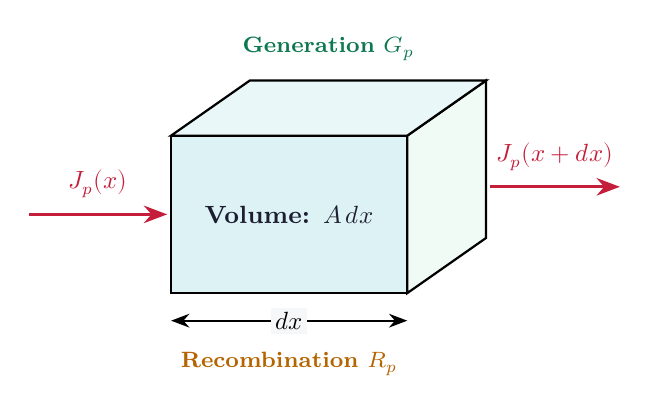
\begin{tikzpicture}[scale=1.0]
  % 3D slab
  \draw[thick, fill=hdrteal] (0,0) rectangle (3.0, 2.0);
  \draw[thick, fill=hdrgreen!40] (3.0,0) -- (4.0, 0.7) -- (4.0, 2.7) -- (3.0, 2.0) -- cycle;
  \draw[thick, fill=hdrteal!60] (0,2.0) -- (1.0, 2.7) -- (4.0, 2.7) -- (3.0, 2.0) -- cycle;

  % Dimension arrows
  \draw[Stealth-Stealth, thick] (0, -0.35) -- (3.0, -0.35) node[midway, fill=mygray, inner sep=1.5pt, font=\small] {$dx$};
  \node[font=\small\bfseries\color{mydark}] at (1.5, 1.0) {Volume: $A\,dx$};

  % Current vectors
  \draw[-Stealth, very thick, color=myred] (-1.8, 1.0) -- (-0.05, 1.0) node[midway, above=2pt, font=\small\bfseries\color{myred}] {$J_p(x)$};
  \draw[-Stealth, very thick, color=myred] (4.05, 1.35) -- (5.7, 1.35) node[midway, above=2pt, font=\small\bfseries\color{myred}] {$J_p(x+dx)$};

  % Generation and Recombination
  \node[font=\footnotesize\bfseries\color{mygreen}] at (2.0, 3.1) {Generation $G_p$};
  \node[font=\footnotesize\bfseries\color{myamber}] at (1.5, -0.9) {Recombination $R_p$};
\end{tikzpicture}
\end{tcolorbox}

The rate of change of total hole charge within the slice must equal the net hole current entering minus exiting, plus generation minus recombination:

\begin{equation}
  \frac{\partial p}{\partial t} A\,dx = \left[ \frac{J_p(x) A}{q} - \frac{J_p(x+dx) A}{q} \right] + (G_p - R_p) A\,dx
\end{equation}

Expanding $J_p(x+dx)$ in a first-order Taylor series:
\begin{equation}
  J_p(x+dx) = J_p(x) + \frac{\partial J_p}{\partial x} dx
\end{equation}

Dividing through by $A\,dx$:

\begin{tcolorbox}[formulabox, title={\textbf{General One-Dimensional Continuity Equations}}]
\begin{align}
  \frac{\partial p}{\partial t} &= -\frac{1}{q} \frac{\partial J_p}{\partial x} + G_p - R_p \quad \text{(Holes)} \\
  \frac{\partial n}{\partial t} &= +\frac{1}{q} \frac{\partial J_n}{\partial x} + G_n - R_n \quad \text{(Electrons)}
\end{align}
\end{tcolorbox}

\subsection{Minority Carrier Diffusion Equation}
Substituting the hole current equation $J_p = q p \mu_p \mathcal{E} - q D_p \frac{\partial p}{\partial x}$ into the continuity equation, setting $R_p - G_{\text{th}} = \frac{\Delta p}{\tau_p}$, and introducing excess optical generation $G_L$:

\begin{equation}
  \frac{\partial (\Delta p)}{\partial t} = D_p \frac{\partial^2 (\Delta p)}{\partial x^2} - \mu_p \mathcal{E} \frac{\partial (\Delta p)}{\partial x} - \mu_p p \frac{\partial \mathcal{E}}{\partial x} + G_L - \frac{\Delta p}{\tau_p}
\end{equation}

For an electric-field-free region ($\mathcal{E} \approx 0$), this simplifies to the celebrated \textbf{Minority Carrier Diffusion Equation}:

\begin{tcolorbox}[formulabox, title={\textbf{Minority Carrier Diffusion Equation (Field-Free Region)}}]
\begin{equation}
  \frac{\partial (\Delta p)}{\partial t} = D_p \frac{\partial^2 (\Delta p)}{\partial x^2} + G_L - \frac{\Delta p}{\tau_p}
\end{equation}
\end{tcolorbox}

\subsubsection{Important Special Case: Steady-State Injection into Semi-Infinite Bar}
Consider a long n-type semiconductor ($x \ge 0$) under steady-state conditions ($\partial/\partial t = 0$), no light ($G_L = 0$), and constant excess hole injection at the surface: $\Delta p(0) = \Delta p_0$. The diffusion equation becomes:

\begin{equation}
  D_p \frac{d^2 (\Delta p)}{dx^2} - \frac{\Delta p}{\tau_p} = 0 \implies \frac{d^2 (\Delta p)}{dx^2} - \frac{\Delta p}{L_p^2} = 0
\end{equation}

Applying boundary conditions:
\begin{itemize}[leftmargin=*, itemsep=2pt]
  \item At $x = 0$: $\Delta p(0) = \Delta p_0$
  \item At $x \to \infty$: $\Delta p(\infty) = 0$
\end{itemize}

The spatial excess carrier profile decays exponentially into the bulk:
\begin{equation}
  \Delta p(x) = \Delta p_0 \exp\left(-\frac{x}{L_p}\right)
\end{equation}
The total injected minority carrier charge per unit area stored in the semiconductor is:
\begin{equation}
  Q_p = q \int_0^\infty \Delta p(x)\,dx = q \Delta p_0 \int_0^\infty e^{-x/L_p}\,dx = q \Delta p_0 L_p
\end{equation}

\newpage
% ===============================================================================
% MANDATORY QUICK REVISION PAGE
% ===============================================================================
\begin{center}
  {\large\bfseries\color{myred} Quick Revision --- Module 1}\\[3pt]
  {\small\color{mydark} Energy Bands \& Current Carriers in Semiconductors $|$ EC301}
\end{center}
\noindent{\color{myred}\rule{\linewidth}{1.2pt}}
\vspace{4pt}

\begin{tcolorbox}[formulabox, title={\textbf{Key Formulas and Metrics at a Glance}}]
\renewcommand{\arraystretch}{1.35}
\begin{tabularx}{\linewidth}{B{5.0cm} X}
Equilibrium Electron Concentration & $n_0 = N_c \exp\left(-\frac{E_c - E_F}{kT}\right)$ \\[4pt]
Equilibrium Hole Concentration & $p_0 = N_v \exp\left(-\frac{E_F - E_v}{kT}\right)$ \\[4pt]
Law of Mass Action & $n_0 p_0 = n_i^2 = N_c N_v \exp\left(-\frac{E_g}{kT}\right)$ \\[4pt]
Intrinsic Fermi Level ($E_i$) & $E_i = \frac{E_c + E_v}{2} + \frac{3}{4} kT \ln\left(\frac{m_h^*}{m_e^*}\right)$ \\[4pt]
Fermi-Dirac Distribution & $f(E) = \frac{1}{1 + \exp\left(\frac{E - E_F}{kT}\right)}$ \\[4pt]
Einstein Relation & $\frac{D_n}{\mu_n} = \frac{D_p}{\mu_p} = \frac{kT}{q} = V_T \approx 25.9\,\text{mV}$ \\[4pt]
Conductivity & $\sigma = q (n\mu_n + p\mu_p)$ \\[4pt]
Total Hole Current Density & $J_p = q p \mu_p \mathcal{E} - q D_p \frac{dp}{dx}$ \\[4pt]
Total Electron Current Density & $J_n = q n \mu_n \mathcal{E} + q D_n \frac{dn}{dx}$ \\[4pt]
Minority Diffusion Length & $L_p = \sqrt{D_p \tau_p}, \quad L_n = \sqrt{D_n \tau_n}$ \\[4pt]
Continuity Equation (Holes) & $\frac{\partial p}{\partial t} = -\frac{1}{q} \frac{\partial J_p}{\partial x} + G_p - R_p$ \\[4pt]
Poisson's Equation & $\frac{d^2 V}{dx^2} = -\frac{q}{\epsilon_s}(p - n + N_D^+ - N_A^-)$ \\[4pt]
\end{tabularx}
\end{tcolorbox}

\begin{tcolorbox}[defbox, title={\textbf{One-Line Definitions}}]
\begin{itemize}[leftmargin=*, itemsep=2pt, topsep=0pt]
  \item \textbf{Covalent Bonding:} Interatomic sharing of valence electron pairs yielding stable octet configurations.
  \item \textbf{Direct Bandgap:} Semiconductor where CB minimum and VB maximum align at the same crystal wavevector ($k=0$).
  \item \textbf{Indirect Bandgap:} Semiconductor where CB minimum is shifted in $k$-space relative to VB maximum, requiring phonon assistance.
  \item \textbf{Fermi Level ($E_F$):} The thermodynamic energy state possessing a $50\%$ probability of occupancy by an electron at $T > 0\,\text{K}$.
  \item \textbf{Intrinsic Semiconductor:} Pure crystalline semiconductor with equal electron and hole concentrations ($n=p=n_i$).
  \item \textbf{Concept of Hole:} Vacant quantum state in the valence band behaving as a mobile positive particle of charge $+q$.
  \item \textbf{Law of Mass Action:} Principle stating that $n_0 p_0 = n_i^2$ is constant at fixed temperature regardless of doping.
  \item \textbf{Carrier Mobility ($\mu$):} Drift velocity per unit applied electric field ($v_d / \mathcal{E}$).
  \item \textbf{Diffusion Length ($L$):} Average distance an injected minority carrier diffuses before recombining.
  \item \textbf{Low-Level Injection:} State where excess injected carrier density is negligible compared to majority carrier concentration.
\end{itemize}
\end{tcolorbox}

\begin{tcolorbox}[exambox, title={\textbf{Frequently Asked / Viva Questions}}]
\begin{enumerate}[topsep=0pt, label=\textbf{Q\arabic*.}, itemsep=5pt]
  \item \Q{Why does Silicon exhibit a negative temperature coefficient of resistance while Copper has a positive one?}
    In semiconductors (Silicon), thermal energy exponentially increases carrier density ($n_i \propto e^{-E_g/2kT}$), which vastly outweighs mobility degradation, making resistance drop ($\text{NTC}$). In metals (Copper), carrier concentration is fixed, and increasing temperature enhances lattice scattering, lowering conductivity ($\text{PTC}$).
  \item \Q{Why is Silicon preferred over Germanium for semiconductor manufacturing?}
    \begin{itemize}[leftmargin=*, itemsep=1pt, topsep=2pt]
      \item Wider bandgap ($1.12\,\text{eV}$ vs $0.66\,\text{eV}$), yielding much lower reverse saturation leakage current ($I_0 \propto n_i^2$).
      \item Higher maximum operating junction temperature ($150^\circ\text{C}$ vs $75^\circ\text{C}$).
      \item Silicon naturally forms a stable, insulating, high-quality native oxide layer ($\text{SiO}_2$), which is critical for planar IC fabrication.
    \end{itemize}
  \item \Q{Why are direct bandgap materials used for LEDs while Silicon is not?}
    In direct bandgap semiconductors ($\text{GaAs}$), electrons transition across the bandgap directly releasing photons without momentum change ($\Delta k = 0$). In Silicon (indirect bandgap), radiative recombination requires a three-particle interaction (electron, hole, phonon), which has extremely low probability; non-radiative thermal dissipation dominates.
  \item \Q{State the Law of Mass Action and its domain of validity.}
    $n_0 p_0 = n_i^2$. It holds strictly under thermal equilibrium in non-degenerate semiconductors. It is invalid under external optical excitation, forward bias injection, or in degenerate semiconductors where $E_F$ enters the bands.
  \item \Q{What is the physical significance of the Einstein Relation?}
    $\frac{D}{\mu} = \frac{kT}{q} = V_T$. It establishes that carrier drift (field-driven transport) and carrier diffusion (thermally driven concentration transport) are fundamentally governed by the same thermal scattering and collision mechanisms.
  \item \Q{Explain the physical meaning of effective mass ($m^*$).}
    Effective mass accounts for the internal periodic potential forces of the crystal lattice on an electron: $m^* = \hbar^2 / \left(\frac{d^2 E}{dk^2}\right)$. It allows Newton's second law ($F = m^* a$) to be applied using only external forces.
  \item \Q{What happens to the Fermi level of an n-type semiconductor as temperature increases to very high values?}
    As temperature increases, intrinsic carrier generation across the bandgap overwhelms donor doping ($n_i \gg N_D$). The semiconductor enters the intrinsic regime, and the Fermi level $E_F$ shifts down from near $E_c$ back toward the intrinsic level $E_i$ (midgap).
  \item \Q{Differentiate between drift and diffusion currents.}
    Drift current is driven by an applied electric field causing directed carrier acceleration. Diffusion current is driven by spatial concentration gradients causing random thermal diffusion from high to low density regions.
  \item \Q{Define minority carrier lifetime and diffusion length.}
    Minority carrier lifetime ($\tau$) is the average time an excess minority carrier survives before recombining. Minority carrier diffusion length ($L = \sqrt{D\tau}$) is the average distance it travels by diffusion during that lifetime.
  \item \Q{What is the significance of the Continuity Equation in semiconductor physics?}
    It enforces the law of conservation of charge carriers across any semiconductor volume element by balancing carrier accumulation against spatial current divergence, net thermal/optical generation, and recombination.
\end{enumerate}
\end{tcolorbox}

\begin{tcolorbox}[tikzbox, title={Comparison of Direct vs. Indirect Bandgap Semiconductors}]
\centering
\renewcommand{\arraystretch}{1.45}
\begin{tabularx}{\linewidth}{|B{3.4cm}|Y|Y|}
\hline
\multicolumn{1}{|c|}{\textbf{Feature}} & \multicolumn{1}{c|}{\textbf{Direct Bandgap}} & \multicolumn{1}{c|}{\textbf{Indirect Bandgap}} \\
\hline
$k$-space Band Alignment & CB minimum and VB maximum occur at identical $k$ ($k=0$) & CB minimum is shifted in $k$-space relative to VB maximum ($k \neq 0$) \\
\hline
Recombination Mechanism & Direct radiative photon emission ($\Delta k = 0$) & Requires simultaneous emission/absorption of a phonon for momentum balance \\
\hline
Radiative Efficiency & Extremely high ($10\%$ to $>50\%$) & Extremely low ($< 0.01\%$, nonradiative dominated) \\
\hline
Carrier Lifetime ($\tau$) & Very short (nanoseconds, $\sim 1\,\text{ns}$ to $10\,\text{ns}$) & Much longer (microseconds, $\sim 1\,\mu\text{s}$ to $1\,\text{ms}$) \\
\hline
Typical Applications & LEDs, Laser Diodes, Photodetectors, High-frequency MMICs & Microprocessors, Memory chips, Power electronic devices \\
\hline
Examples & $\text{GaAs}$, $\text{InP}$, $\text{GaN}$, $\text{InGaAs}$ & $\text{Si}$, $\text{Ge}$, $\text{AlAs}$, $\text{GaP}$ \\
\hline
\end{tabularx}
\end{tcolorbox}


% -- Module 2 -----------------------------------------------------------------
\modulestart{2}{Physical Description of the P-N Junction}

\section{Physical Description of the P-N Junction}
% ===============================================================================

A \textbf{p-n junction} is formed when a p-type semiconductor material is joined seamlessly at an atomic level with an n-type semiconductor material within a single continuous crystal lattice.

\subsection{Thermal Equilibrium and Depletion Region Formation}
Due to the steep concentration gradients across the metallurgical junction ($x = 0$):
\begin{itemize}[leftmargin=*, itemsep=3pt]
  \item Majority holes in the p-region diffuse across the interface into the n-region, where they recombine with majority electrons.
  \item Majority electrons in the n-region diffuse into the p-region and recombine with holes.
  \item This diffusion uncovers uncompensated, immobile ionized dopant cores:
    \begin{itemize}
      \item Negatively charged acceptor ions ($N_A^-$) in the p-side ($ -x_p \le x \le 0 $).
      \item Positively charged donor ions ($N_D^+$) in the n-side ($ 0 \le x \le x_n $).
    \end{itemize}
  \item The region containing these uncovered unneutralized fixed charges is devoid of mobile carriers and is called the \textbf{depletion region} (or \textbf{space charge region}).
  \item The fixed charges establish an internal electric field $\vec{\mathcal{E}}$ pointing from the positive donor ions ($+x$) to the negative acceptor ions ($-x$). This field exerts a drift force that opposes further carrier diffusion.
  \item At \textbf{thermal equilibrium}, the drift current driven by $\vec{\mathcal{E}}$ exactly balances the diffusion current driven by concentration gradients, resulting in zero net current:
  \begin{equation}
    J_n = J_{n,\text{drift}} + J_{n,\text{diff}} = 0, \qquad J_p = J_{p,\text{drift}} + J_{p,\text{diff}} = 0
  \end{equation}
\end{itemize}

\begin{tcolorbox}[tikzbox, title={Space Charge Region and Charge Density Profile of an Abrupt P-N Junction}]
\centering
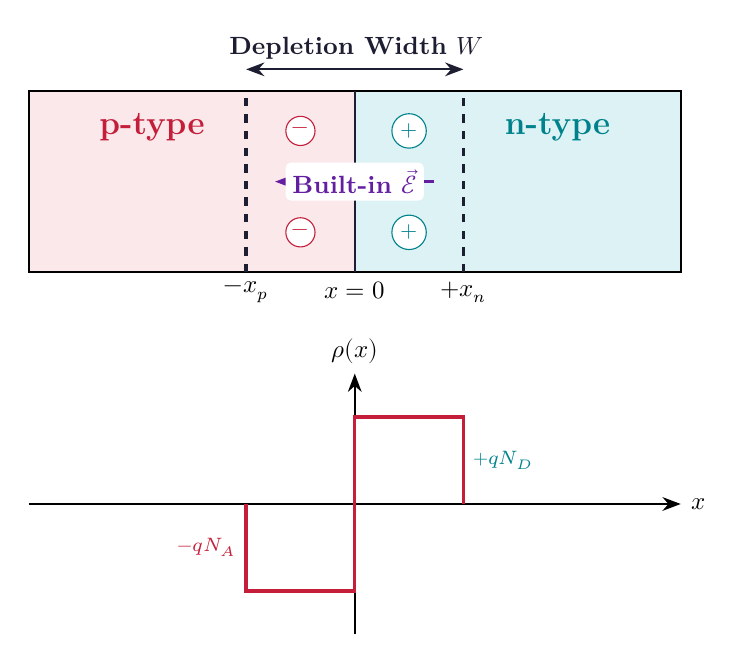
\begin{tikzpicture}[scale=0.92]
  % P and N regions
  \draw[thick, fill=hdrred] (-4.5, 0) rectangle (0, 2.5);
  \draw[thick, fill=hdrteal] (0, 0) rectangle (4.5, 2.5);
  \node[font=\large\bfseries\color{myred}] at (-2.8, 2.0) {p-type};
  \node[font=\large\bfseries\color{myteal}] at (2.8, 2.0) {n-type};

  % Depletion boundaries
  \draw[dashed, very thick, color=mydark] (-1.5, 0) -- (-1.5, 2.5);
  \draw[dashed, very thick, color=mydark] (1.5, 0) -- (1.5, 2.5);
  \draw[thick, color=mydark] (0, 0) -- (0, 2.5);

  % Immobile ions
  \foreach \y in {0.55, 1.95} {
    \node[draw=myred, circle, inner sep=1.5pt, fill=white, font=\footnotesize\bfseries\color{myred}] at (-0.75, \y) {$-$};
    \node[draw=myteal, circle, inner sep=1.5pt, fill=white, font=\footnotesize\bfseries\color{myteal}] at (0.75, \y) {$+$};
  }

  % Electric field vector
  \draw[-Stealth, very thick, color=mypurple] (1.1, 1.25) -- (-1.1, 1.25) node[midway, fill=white, inner sep=2.5pt, rounded corners=2pt, font=\small\bfseries\color{mypurple}] {Built-in $\vec{\mathcal{E}}$};

  % Labels
  \node[below, font=\small] at (-1.5, 0) {$-x_p$};
  \node[below, font=\small] at (0, 0) {$x=0$};
  \node[below, font=\small] at (1.5, 0) {$+x_n$};
  \draw[Stealth-Stealth, thick, color=mydark] (-1.5, 2.8) -- (1.5, 2.8) node[midway, above, font=\small\bfseries] {Depletion Width $W$};

  % Space charge density plot rho(x)
  \begin{scope}[yshift=-3.2cm]
    \draw[-Stealth, thick] (-4.5, 0) -- (4.5, 0) node[right, font=\small] {$x$};
    \draw[-Stealth, thick] (0, -1.8) -- (0, 1.8) node[above, font=\small] {$\rho(x)$};
    \draw[very thick, color=myred] (-1.5, 0) -- (-1.5, -1.2) -- (0, -1.2) -- (0, 1.2) -- (1.5, 1.2) -- (1.5, 0);
    \node[left, font=\scriptsize\bfseries\color{myred}] at (-1.5, -0.6) {$-q N_A$};
    \node[right, font=\scriptsize\bfseries\color{myteal}] at (1.5, 0.6) {$+q N_D$};
  \end{scope}
\end{tikzpicture}
\end{tcolorbox}

\subsection{Derivation of the Built-In Potential (\texorpdfstring{$V_{bi}$}{Vbi})}
Under thermal equilibrium, setting the hole current density to zero:
\begin{align}
  J_p = q p \mu_p \mathcal{E} - q D_p \frac{dp}{dx} &= 0 \\
  \mu_p \mathcal{E} &= D_p \frac{1}{p} \frac{dp}{dx}
\end{align}

Using the Einstein relation $\frac{D_p}{\mu_p} = \frac{kT}{q} = V_T$ and the electrostatic relation $\mathcal{E} = -\frac{dV}{dx}$:
\begin{equation}
  -\frac{dV}{dx} = \frac{k T}{q} \frac{1}{p} \frac{dp}{dx} \implies -dV = \frac{k T}{q} \frac{dp}{p}
\end{equation}

Integrating from the neutral p-region ($x = -x_p$, where $p = p_{p0} \approx N_A$ and $V = 0$) to the neutral n-region ($x = x_n$, where $p = p_{n0} = n_i^2/N_D$ and $V = V_{bi}$):
\begin{equation}
  -\int_0^{V_{bi}} dV = \frac{k T}{q} \int_{p_{p0}}^{p_{n0}} \frac{dp}{p}
\end{equation}
\begin{equation}
  -V_{bi} = \frac{k T}{q} \ln\left(\frac{p_{n0}}{p_{p0}}\right) = -\frac{k T}{q} \ln\left(\frac{p_{p0}}{p_{n0}}\right)
\end{equation}

Substituting $p_{p0} \approx N_A$ and $p_{n0} = \frac{n_i^2}{N_D}$:

\begin{tcolorbox}[formulabox, title={\textbf{Built-In Potential (Contact Potential)}}]
\begin{equation}
  V_{bi} = V_T \ln\left(\frac{N_A N_D}{n_i^2}\right) = \frac{k T}{q} \ln\left(\frac{N_A N_D}{n_i^2}\right)
\end{equation}
At $T = 300\,\text{K}$ ($V_T \approx 25.9\,\text{mV}$), for Silicon with $N_A = 10^{16}\,\text{cm}^{-3}, N_D = 10^{17}\,\text{cm}^{-3}$:
$V_{bi} \approx 0.0259 \ln\left(\frac{10^{33}}{2.25 \times 10^{20}}\right) \approx 0.75\,\text{V}$.
\end{tcolorbox}

\subsection{Depletion Width and Electric Field Analysis}
By integrating Poisson's equation $\frac{d\mathcal{E}}{dx} = \frac{\rho(x)}{\epsilon_s}$ across an abrupt step junction:
\begin{itemize}[leftmargin=*, itemsep=2pt]
  \item For $-x_p \le x \le 0$: $\mathcal{E}(x) = -\frac{q N_A}{\epsilon_s} (x + x_p)$
  \item For $0 \le x \le x_n$: $\mathcal{E}(x) = +\frac{q N_D}{\epsilon_s} (x - x_n)$
\end{itemize}

By overall charge neutrality, the total negative space charge must balance the positive space charge:
\begin{equation}
  q N_A x_p = q N_D x_n \implies \frac{x_n}{x_p} = \frac{N_A}{N_D}
\end{equation}
The depletion region penetrates deeper into the more lightly doped semiconductor side.

\begin{tcolorbox}[formulabox, title={\textbf{Depletion Width and Peak Electric Field under Applied Bias $V_a$}}]
For an applied voltage $V_a$ ($V_a > 0$ for forward bias, $V_a = -V_R$ for reverse bias):
\begin{equation}
  W = x_n + x_p = \sqrt{\frac{2 \epsilon_s}{q} \left(\frac{1}{N_A} + \frac{1}{N_D}\right) (V_{bi} - V_a)}
\end{equation}
Individual depletion layer penetrations:
\begin{equation}
  x_n = W \left(\frac{N_A}{N_A + N_D}\right), \qquad x_p = W \left(\frac{N_D}{N_A + N_D}\right)
\end{equation}
The maximum electric field occurs at the metallurgical junction ($x = 0$):
\begin{equation}
  \mathcal{E}_{\text{max}} = -\frac{2 (V_{bi} - V_a)}{W} = -\frac{q N_D x_n}{\epsilon_s} = -\frac{q N_A x_p}{\epsilon_s}
\end{equation}
\end{tcolorbox}

\subsection{Energy Band Diagrams under Bias}
\begin{itemize}[leftmargin=*, itemsep=3pt]
  \item \textbf{Thermal Equilibrium ($V_a = 0$):} The Fermi level is flat throughout the entire device ($dE_F/dx = 0$). The total band bending is equal to the built-in potential barrier: $q V_{bi}$.
  \item \textbf{Forward Bias ($V_a > 0$):} Positive terminal connected to p-side, negative to n-side. The potential barrier is reduced to $q(V_{bi} - V_a)$. Depletion width narrows, and the Fermi level splits into two separate \textbf{quasi-Fermi levels}: $E_{Fn} - E_{Fp} = q V_a$. Majority carriers readily diffuse across the lowered barrier.
  \item \textbf{Reverse Bias ($V_a = -V_R < 0$):} Positive terminal connected to n-side, negative to p-side. The potential barrier increases to $q(V_{bi} + V_R)$. Depletion width expands, completely blocking majority diffusion. Only thermally generated minority carriers drift across the junction, producing a tiny saturation current $I_0$.
\end{itemize}

% ===============================================================================
\section{P-N Junction Fabrication Technologies}
% ===============================================================================

Modern semiconductor devices are fabricated using planar integrated circuit technologies:

\par\vspace{6pt}\noindent
\begingroup
\setlength{\tabcolsep}{5pt}
\setlength{\extrarowheight}{3pt}
\renewcommand{\arraystretch}{1.35}
\begin{tabularx}{\linewidth}{|B{3.2cm}|Y|Y|}
\hline
\multicolumn{1}{|c|}{\textbf{Method}} & \multicolumn{1}{c|}{\textbf{Process Description}} & \multicolumn{1}{c|}{\textbf{Key Characteristics}} \\
\hline
Grown Junction & Dopant impurities are introduced into the molten melt during crystal pulling (Czochralski process). & Historical method; poor dimensional control; abruptness limited. \\
\hline
Alloyed Junction & A pellet of trivalent impurity (e.g., Indium) is melted onto an n-type substrate and recrystallized. & Forms extremely abrupt junctions; rugged; large junction depth variations. \\
\hline
Thermal Diffusion & Dopant vapor is diffused at elevated temperatures ($900\text{--}1200^\circ\text{C}$) into masked wafer windows. & Planar geometry; excellent reproducibility; lateral diffusion under oxide masks occurs. \\
\hline
Ion Implantation & Dopant ions are ionized, accelerated to high energies ($10\text{--}400\,\text{keV}$), and fired into the wafer. & Precise dosage and depth profile control; low processing temperature; requires thermal annealing to heal crystal damage. \\
\hline
Epitaxial Growth & High-purity single-crystal layer grown on single-crystal substrate using Chemical Vapor Deposition (CVD). & Controlled uniform thickness and doping; used for collector layers and buried layers. \\
\hline
\end{tabularx}
\endgroup

% ===============================================================================
\section{I-V Characteristics and Small Signal Switching Models}
% ===============================================================================

\subsection{The Shockley Diode Equation}
Under the assumption of low-level injection and steady-state conditions, the current flowing through a p-n junction diode is given by the \textbf{Shockley Ideal Diode Equation}:

\begin{tcolorbox}[formulabox, title={\textbf{Shockley Diode Equation and Reverse Saturation Current}}]
\begin{equation}
  I = I_0 \left[ \exp\left(\frac{q V_a}{\eta k T}\right) - 1 \right] = I_0 \left[ \exp\left(\frac{V_a}{\eta V_T}\right) - 1 \right]
\end{equation}
where $\eta$ is the \textbf{ideality factor} ($\eta \approx 1$ for Germanium; $\eta \approx 2$ at low current in Silicon where depletion recombination dominates, and $\eta \approx 1$ at higher forward currents where diffusion dominates).

The \textbf{reverse saturation current} $I_0$ is:
\begin{equation}
  I_0 = q A \left( \frac{D_p p_{n0}}{L_p} + \frac{D_n n_{p0}}{L_n} \right) = q A n_i^2 \left( \frac{D_p}{L_p N_D} + \frac{D_n}{L_n N_A} \right)
\end{equation}
Because $I_0 \propto n_i^2 \propto T^3 \exp(-E_g / kT)$, $I_0$ is extremely temperature-sensitive:
\begin{itemize}[leftmargin=*, itemsep=2pt, topsep=0pt]
  \item $I_0$ approximately \textbf{doubles for every $10^\circ\text{C}$ rise} in temperature for Silicon.
  \item Forward voltage drop decreases by approximately $\mathbf{-2\,\text{mV/}^\circ\text{C}}$ for a constant forward current.
\end{itemize}
\end{tcolorbox}

\subsection{Small-Signal AC Model of P-N Diode}
When a small sinusoidal AC signal ($v_d \ll V_T$) is superimposed on a DC operating point ($V_D, I_D$):

\begin{enumerate}[label=\arabic*., leftmargin=*]
  \item \textbf{Dynamic (AC) Resistance ($r_d$):} The slope of the forward I-V characteristic:
  \begin{equation}
    r_d = \left(\frac{dI}{dV}\right)^{-1} = \frac{\eta V_T}{I_D + I_0} \approx \frac{\eta V_T}{I_D}
  \end{equation}
  At $I_D = 1\,\text{mA}$, for $\eta = 1$: $r_d \approx \frac{25.9\,\text{mV}}{1\,\text{mA}} \approx 26\,\Omega$.

  \item \textbf{Junction (Depletion) Capacitance ($C_j$):} Arises from dipole charge variation ($dQ/dV$) stored in the uncompensated depletion region under reverse bias:
  \begin{equation}
    C_j = \frac{\epsilon_s A}{W} = \frac{C_{j0}}{\left(1 + \displaystyle\frac{V_R}{V_{bi}}\right)^m}
  \end{equation}
  where $m = 1/2$ for an abrupt (step) junction, and $m = 1/3$ for a linearly graded junction. Dominates under \textbf{reverse bias}.

  \item \textbf{Diffusion Capacitance ($C_d$):} Arises from the rearrangement of injected excess minority carrier charge stored in the neutral regions under forward bias:
  \begin{equation}
    C_d = \frac{d Q_{\text{diff}}}{d V_a} = \frac{d (I_D \tau_T)}{d V_a} = \tau_T \frac{d I_D}{d V_a} = \frac{\tau_T I_D}{\eta V_T}
  \end{equation}
  where $\tau_T$ is the minority carrier transit time. $C_d$ is directly proportional to forward current $I_D$ and dominates heavily under \textbf{forward bias}.
\end{enumerate}

\subsection{Diode Switching Characteristics and Reverse Recovery Time}
When a diode is switched rapidly from forward conduction ($I_F$) to reverse bias ($-V_R$):

\begin{itemize}[leftmargin=*, itemsep=3pt]
  \item The diode cannot turn off instantaneously because a substantial amount of excess minority carrier charge $Q_s = I_F \tau_T$ is stored in the neutral base.
  \item \textbf{Storage Time ($t_s$):} The time required to extract the stored excess charge near the junction until the carrier density drops to equilibrium. Current remains high and negative ($I_R \approx -V_R / R_L$).
  \item \textbf{Transition Time ($t_t$):} The time required for the junction depletion layer capacitance to charge up to the reverse bias voltage $-V_R$. Current decays asymptotically to $-I_0$.
  \item \textbf{Reverse Recovery Time ($t_{rr}$):} Total turn-off time:
  \begin{equation}
    t_{rr} = t_s + t_t
  \end{equation}
\end{itemize}

% ===============================================================================
\section{Junction Breakdown Mechanisms and Diodes}
% ===============================================================================

When a sufficiently large reverse bias voltage ($V_R = V_{BR}$) is applied across a p-n junction, the reverse current increases drastically with negligible increase in voltage.

\subsection{Zener Breakdown vs. Avalanche Breakdown}
\par\vspace{6pt}\noindent
\begingroup
\setlength{\tabcolsep}{5pt}
\setlength{\extrarowheight}{3pt}
\renewcommand{\arraystretch}{1.35}
\begin{tabularx}{\linewidth}{|B{3.2cm}|Y|Y|}
\hline
\multicolumn{1}{|c|}{\textbf{Parameter}} & \multicolumn{1}{c|}{\textbf{Zener Breakdown}} & \multicolumn{1}{c|}{\textbf{Avalanche Breakdown}} \\
\hline
Doping Concentration & Heavily doped on both p and n sides ($N_A, N_D > 10^{18}\,\text{cm}^{-3}$) & Lightly to moderately doped ($N_A, N_D < 10^{16}\,\text{cm}^{-3}$) \\
\hline
Depletion Width ($W$) & Extremely thin ($W < 10\,\text{nm} = 100\,\text{\AA}$) & Relatively wide ($W > 1\,\mu\text{m}$) \\
\hline
Breakdown Voltage ($V_{BR}$) & Occurs at low reverse voltages ($V_{BR} < 4\text{--}6\,\text{V}$) & Occurs at higher reverse voltages ($V_{BR} > 6\,\text{V}$) \\
\hline
Physical Mechanism & Direct quantum mechanical tunneling of valence electrons from p-side VB to n-side CB across thin barrier & Impact ionization: high kinetic energy carriers collide with lattice atoms, generating secondary EHPs (avalanche multiplication) \\
\hline
Electric Field & High electric field ($\mathcal{E} \ge 10^6\,\text{V/cm}$) & Moderate to high field ($\mathcal{E} \sim 2\text{--}4 \times 10^5\,\text{V/cm}$) \\
\hline
Temperature Coefficient & \textbf{Negative:} As $T$ rises, bandgap $E_g$ narrows, making tunneling easier $\implies V_Z$ decreases & \textbf{Positive:} As $T$ rises, lattice vibrations increase, shortening mean free path, requiring higher voltage for collision ionization $\implies V_A$ increases \\
\hline
\end{tabularx}
\endgroup

\subsection{Schottky Diode (Metal-Semiconductor Junction)}
A \textbf{Schottky barrier diode} is formed by depositing a metal (e.g., Gold, Platinum, Tungsten, Aluminum) directly onto an n-type semiconductor.

\begin{itemize}[leftmargin=*, itemsep=3pt]
  \item \textbf{Schottky Barrier Height ($\Phi_B$):}
  \begin{equation}
    \Phi_B = \Phi_m - \chi_s
  \end{equation}
  where $\Phi_m$ is the metal work function, and $\chi_s$ is the semiconductor electron affinity.
  \item \textbf{Built-in Potential ($V_{bi}$):}
  \begin{equation}
    V_{bi} = \Phi_B - (E_c - E_F) / q
  \end{equation}
  \item \textbf{Majority Carrier Conduction:} Current conduction occurs entirely via majority electron \textbf{thermionic emission} over the barrier into the metal.
  \item \textbf{Zero Minority Storage Time:} Because there is virtually no minority carrier injection into the semiconductor, there is zero stored charge ($Q_s \approx 0$). The reverse recovery time $t_{rr}$ is virtually zero ($\sim 10\text{--}100\,\text{ps}$), making Schottky diodes ideal for high-speed switching and ultra-high frequency (RF/microwave) clamping circuits.
  \item \textbf{Low Cut-In Voltage:} The forward knee voltage is only $0.2\text{--}0.3\,\text{V}$ (compared to $0.7\,\text{V}$ for Silicon p-n diodes).
\end{itemize}

% ===============================================================================
\section{Bipolar Junction Transistor (BJT)}
% ===============================================================================

The Bipolar Junction Transistor is a three-terminal, two-junction semiconductor device whose operation depends on both majority and minority carrier transport (hence \textbf{bipolar}).

\subsection{Basic Construction and Doping Asymmetry}
A BJT consists of three alternating regions: Emitter ($E$), Base ($B$), and Collector ($C$), forming an n-p-n or p-n-p sandwich:

\par\vspace{6pt}\noindent
\begingroup
\setlength{\tabcolsep}{3.5pt}
\setlength{\extrarowheight}{3pt}
\renewcommand{\arraystretch}{1.35}
\begin{tabularx}{\linewidth}{|B{2.2cm}|Y|Y|Y|}
\hline
\textbf{Region} & \textbf{Doping Concentration} & \textbf{Physical Width} & \textbf{Primary Functional Role} \\
\hline
Emitter ($E$) & Heavily doped ($N_E \approx 10^{19}\,\text{cm}^{-3}$) & Moderate & Injects majority carriers into the base with maximum injection efficiency. \\
\hline
Base ($B$) & Very lightly doped ($N_B \approx 10^{16}\,\text{cm}^{-3}$) & Extremely narrow ($W_b \ll L_{\text{minority}}$) & Transports injected minority carriers to the collector with minimum recombination. \\
\hline
Collector ($C$) & Moderately / Lightly doped ($N_C \approx 10^{15}\,\text{cm}^{-3}$) & Largest physical dimensions & Collects carriers sweeping across reverse-biased CB junction; dissipates heat. \\
\hline
\end{tabularx}
\endgroup

\subsection{BJT Operating Modes}
\par\vspace{6pt}\noindent
\begingroup
\setlength{\tabcolsep}{3.5pt}
\setlength{\extrarowheight}{3pt}
\renewcommand{\arraystretch}{1.35}
\begin{tabularx}{\linewidth}{|B{2.3cm}|Y|Y|Y|}
\hline
\textbf{Operating Mode} & \textbf{Emitter-Base Junction (EBJ)} & \textbf{Collector-Base Junction (CBJ)} & \textbf{Primary Application} \\
\hline
Forward Active & Forward Biased & Reverse Biased & Linear analog amplification \\
\hline
Cut-off & Reverse Biased & Reverse Biased & Digital logic ``OFF'' switch ($I_C \approx 0$) \\
\hline
Saturation & Forward Biased & Forward Biased & Digital logic ``ON'' switch ($V_{CE,\text{sat}} \approx 0.2\,\text{V}$) \\
\hline
Inverse / Inverted & Reverse Biased & Forward Biased & Specialized bidirectional switching \\
\hline
\end{tabularx}
\endgroup

\subsection{Current Relationships in Forward Active Mode}
For an n-p-n transistor in forward active mode:
\begin{enumerate}[label=\arabic*., leftmargin=*]
  \item Electrons injected from Emitter into Base form emitter current $I_E$.
  \item A tiny fraction ($< 1\%$) recombines with holes in the thin base, forming base current $I_B$.
  \item The remaining vast majority ($> 99\%$) diffuses across the neutral base, reaches the CB depletion edge, and is swept into the collector by the strong reverse electric field, forming collector current $I_C$:
\end{enumerate}

\begin{tcolorbox}[formulabox, title={\textbf{BJT Current Relationships}}]
\begin{equation}
  I_E = I_B + I_C
\end{equation}
Common-Base Current Gain ($\alpha$):
\begin{equation}
  \alpha = \frac{I_C}{I_E} \approx 0.95 \text{ to } 0.998
\end{equation}
Common-Emitter Current Gain ($\beta$ or $h_{FE}$):
\begin{equation}
  \beta = \frac{I_C}{I_B} = \frac{\alpha}{1 - \alpha} \approx 50 \text{ to } 500
\end{equation}
In terms of reverse collector saturation current ($I_{CBO}$):
\begin{equation}
  I_C = \alpha I_E + I_{CBO} = \beta I_B + (\beta + 1) I_{CBO} = \beta I_B + I_{CEO}
\end{equation}
\end{tcolorbox}

\subsection{Base Width Modulation (The Early Effect)}
In forward active mode, as the reverse bias voltage across the collector-base junction ($V_{CB}$ or $V_{CE}$) increases:
\begin{itemize}[leftmargin=*, itemsep=3pt]
  \item The collector-base space charge region expands into the lightly doped base.
  \item The \textbf{effective neutral base width} ($W_{\text{eff}} = W_{\text{base}} - x_{p,\text{dep}}$) decreases.
  \item \textbf{Consequences}:
    \begin{enumerate}
      \item Less recombination in the base $\implies$ Base transport factor increases $\implies \alpha$ and $\beta$ increase.
      \item The concentration gradient of minority electrons in the base ($dn/dx \approx n(0)/W_{\text{eff}}$) steepens $\implies I_C$ increases with increasing $V_{CE}$.
    \end{enumerate}
  \item When extrapolated backward, the linear output characteristics in the active region intersect the negative voltage axis at a common voltage called the \textbf{Early Voltage} ($V_A \approx 50\text{--}100\,\text{V}$).
  \item The collector current incorporating the Early effect is modeled as:
  \begin{equation}
    I_C = I_S \exp\left(\frac{V_{BE}}{V_T}\right) \left( 1 + \frac{V_{CE}}{V_A} \right)
  \end{equation}
  yielding a finite small-signal output resistance: $r_o = \frac{V_A + V_{CE}}{I_C} \approx \frac{V_A}{I_C}$.
\end{itemize}

\subsection{BJT I-V Characteristics (Common-Emitter Input and Output)}
The static electrical behavior of a BJT in the Common-Emitter (CE) configuration is described by two sets of characteristic curves:

\begin{enumerate}[label=\arabic*., leftmargin=*]
  \item \textbf{Input Characteristics ($I_B$ vs. $V_{BE}$ for constant $V_{CE}$):}
  \begin{itemize}
    \item Resembles the exponential forward $I\text{-}V$ curve of a p-n junction diode with knee / cut-in voltage $V_\gamma \approx 0.6\text{--}0.7\,\text{V}$ for Silicon.
    \item As $V_{CE}$ increases, base width modulation (Early effect) narrows the effective base width $W_{\text{eff}}$, reducing base recombination. Consequently, a higher $V_{BE}$ is required to sustain the same base current $I_B$, shifting the curve slightly to the right.
    \item \textbf{Dynamic Input Resistance:} $h_{ie} = r_\pi = \left.\frac{\partial V_{BE}}{\partial I_B}\right|_{V_{CE} = \text{const}} \approx 1\text{ to } 5\,\text{k}\Omega$.
  \end{itemize}
  \item \textbf{Output Characteristics ($I_C$ vs. $V_{CE}$ for constant $I_B$):}
  Displays four distinct regions of transistor operation:
  \begin{itemize}
    \item \textbf{Cut-off Region ($I_B \le 0$):} Both EBJ and CBJ are reverse-biased. The transistor is turned OFF, with only a negligible leakage current flowing: $I_C = I_{CEO} = (\beta + 1)I_{CBO} \approx 0$.
    \item \textbf{Saturation Region ($0 \le V_{CE} \le V_{CE,\text{sat}} \approx 0.2\,\text{V}$):} Both EBJ and CBJ are forward-biased. $I_C$ increases rapidly and linearly with $V_{CE}$, limited only by external circuit load ($I_{C,\text{sat}} \approx V_{CC}/R_C$), independent of $I_B$ ($I_C < \beta I_B$).
    \item \textbf{Active Region ($V_{CE} > 0.2\,\text{V}$, $I_B > 0$):} EBJ is forward-biased and CBJ is reverse-biased. The collector current is controlled primarily by the base current ($I_C \approx \beta I_B$). Curves exhibit a slight positive slope due to Early effect, with an output resistance $r_o = \left.\frac{\partial V_{CE}}{\partial I_C}\right|_{I_B} \approx \frac{V_A}{I_C} \approx 40\text{--}100\,\text{k}\Omega$.
    \item \textbf{Avalanche Breakdown Region ($V_{CE} > BV_{CEO}$):} The reverse-biased CB junction enters avalanche multiplication, causing $I_C$ to rise steeply and destructively.
  \end{itemize}
\end{enumerate}

\begin{tcolorbox}[tikzbox, title={Common-Emitter (CE) Output Characteristics ($I_C$ vs. $V_{CE}$)}]
\centering
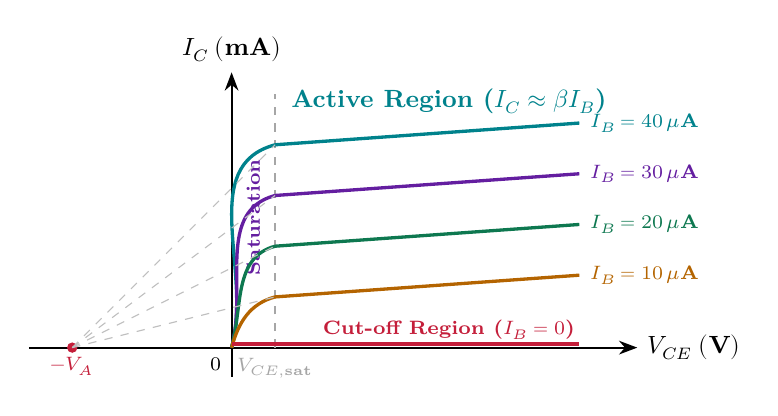
\begin{tikzpicture}[scale=0.92]
  % Axes
  \draw[-Stealth, thick] (-2.8, 0) -- (5.6, 0) node[right, font=\small\bfseries] {$V_{CE}\;(\text{V})$};
  \draw[-Stealth, thick] (0, -0.4) -- (0, 3.8) node[above, font=\small\bfseries] {$I_C\;(\text{mA})$};
  \node[below left, font=\scriptsize] at (0,0) {$0$};

  % Saturation boundary line
  \draw[dashed, thick, color=gray!70] (0.6, 0) node[below, font=\scriptsize\bfseries\color{mydark}] {$V_{CE,\text{sat}}$} -- (0.6, 3.5);

  % Region labels
  \node[font=\scriptsize\bfseries\color{mypurple}, rotate=90] at (0.3, 1.8) {Saturation};
  \node[font=\small\bfseries\color{myteal}] at (3.0, 3.4) {Active Region ($I_C \approx \beta I_B$)};
  \node[font=\scriptsize\bfseries\color{myred}] at (3.0, 0.25) {Cut-off Region ($I_B = 0$)};

  % Early voltage extrapolation point
  \filldraw[color=myred] (-2.2, 0) circle (1.8pt) node[below, font=\scriptsize\bfseries\color{myred}] {$-V_A$};

  % I_B curves
  \foreach \ib/\yc/\col in {40/2.8/myteal, 30/2.1/mypurple, 20/1.4/mygreen, 10/0.7/myamber} {
    \draw[very thick, color=\col] (0,0) to[out=75, in=195] (0.6, \yc);
    \draw[very thick, color=\col] (0.6, \yc) -- (4.8, \yc + 0.3) node[right, font=\scriptsize\bfseries] {$I_B = \ib\,\mu\text{A}$};
    \draw[dashed, thin, color=gray!50] (-2.2, 0) -- (0.6, \yc);
  }

  % Cut-off curve
  \draw[very thick, color=myred] (0, 0.05) -- (4.8, 0.05);
\end{tikzpicture}
\end{tcolorbox}

% ===============================================================================
\section{The Ebers-Moll Model}
% ===============================================================================

The \textbf{Ebers-Moll model} is a generalized, physics-based, large-signal non-linear equivalent circuit model for the BJT valid across \textbf{all four operating modes} (Active, Cut-off, Saturation, and Inverted).

\subsection{Model Formulation and Equivalent Circuit}
The BJT is modeled as two coupled p-n junction diodes connected back-to-back with two current-controlled current sources representing the transistor action:

\begin{itemize}[leftmargin=*, itemsep=3pt]
  \item An Emitter diode carrying current $I_F$ with a dependent collector current source $\alpha_F I_F$.
  \item A Collector diode carrying current $I_R$ with a dependent emitter current source $\alpha_R I_R$.
\end{itemize}

where:
\begin{align}
  I_F &= I_{ES} \left[ \exp\left(\frac{q V_{BE}}{k T}\right) - 1 \right] \\
  I_R &= I_{CS} \left[ \exp\left(\frac{q V_{BC}}{k T}\right) - 1 \right]
\end{align}
$I_{ES}$ and $I_{CS}$ are the saturation currents of the Emitter-Base and Collector-Base junctions, respectively, and $\alpha_F$ ($\alpha_{\text{forward}}$) and $\alpha_R$ ($\alpha_{\text{reverse}}$) are the forward and reverse common-base current gains.

\begin{tcolorbox}[formulabox, title={\textbf{Ebers-Moll Equations}}]
The terminal currents for an n-p-n transistor are:
\begin{align}
  I_E &= I_F - \alpha_R I_R = I_{ES} \left( e^{V_{BE}/V_T} - 1 \right) - \alpha_R I_{CS} \left( e^{V_{BC}/V_T} - 1 \right) \\
  I_C &= \alpha_F I_F - I_R = \alpha_F I_{ES} \left( e^{V_{BE}/V_T} - 1 \right) - I_{CS} \left( e^{V_{BC}/V_T} - 1 \right) \\
  I_B &= I_E - I_C = (1 - \alpha_F) I_F + (1 - \alpha_R) I_R
\end{align}
\textbf{The Reciprocity Condition:} By thermodynamic reciprocity of linear carrier diffusion across the base:
\begin{equation}
  \alpha_F I_{ES} = \alpha_R I_{CS} = I_S
\end{equation}
where $I_S$ is the fundamental BJT saturation transfer current.
\end{tcolorbox}

\begin{tcolorbox}[tikzbox, title={Ebers-Moll Large-Signal Equivalent Circuit (N-P-N Transistor)}]
\centering
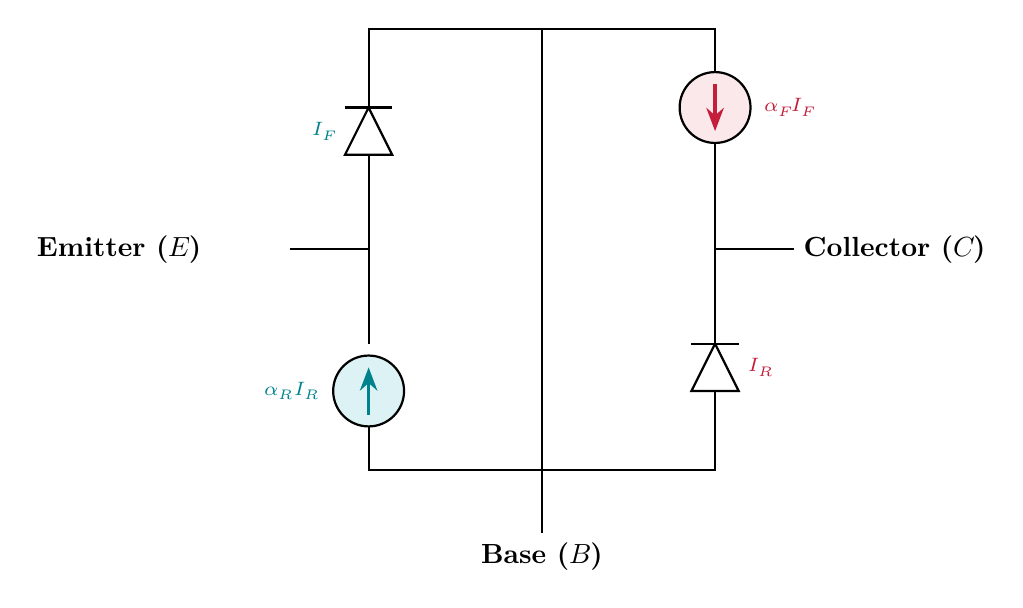
\begin{tikzpicture}[scale=1.0]
  % Emitter Terminal
  \node[left, font=\normalsize\bfseries] at (-4.2, 0) {Emitter ($E$)};
  \draw[thick] (-3.2, 0) -- (-2.2, 0);

  % Forward Diode
  \draw[thick] (-2.2, 0) -- (-2.2, 1.2);
  \draw[thick] (-2.5, 1.2) -- (-1.9, 1.2) -- (-2.2, 1.8) -- cycle;
  \draw[thick] (-2.5, 1.8) -- (-1.9, 1.8);
  \draw[thick] (-2.2, 1.8) -- (-2.2, 2.8) -- (0, 2.8);
  \node[left, font=\scriptsize\bfseries\color{myteal}] at (-2.5, 1.5) {$I_F$};

  % Reverse Current Source alpha_R * I_R
  \draw[thick] (-2.2, 0) -- (-2.2, -1.2);
  \draw[thick, fill=hdrteal] (-2.2, -1.8) circle (0.45);
  \draw[-Stealth, very thick, color=myteal] (-2.2, -2.1) -- (-2.2, -1.5);
  \node[left, font=\scriptsize\bfseries\color{myteal}] at (-2.7, -1.8) {$\alpha_R I_R$};
  \draw[thick] (-2.2, -2.25) -- (-2.2, -2.8) -- (0, -2.8);

  % Base Terminal
  \draw[thick] (0, 2.8) -- (0, -2.8);
  \draw[thick] (0, 0) -- (0, -3.6) node[below, font=\normalsize\bfseries] {Base ($B$)};

  % Forward Current Source alpha_F * I_F
  \draw[thick] (0, 2.8) -- (2.2, 2.8) -- (2.2, 2.25);
  \draw[thick, fill=hdrred] (2.2, 1.8) circle (0.45);
  \draw[-Stealth, very thick, color=myred] (2.2, 2.1) -- (2.2, 1.5);
  \node[right, font=\scriptsize\bfseries\color{myred}] at (2.7, 1.8) {$\alpha_F I_F$};
  \draw[thick] (2.2, 1.35) -- (2.2, 0);

  % Reverse Diode
  \draw[thick] (0, -2.8) -- (2.2, -2.8) -- (2.2, -1.8);
  \draw[thick] (1.9, -1.8) -- (2.5, -1.8) -- (2.2, -1.2) -- cycle;
  \draw[thick] (1.9, -1.2) -- (2.5, -1.2);
  \draw[thick] (2.2, -1.2) -- (2.2, 0);
  \node[right, font=\scriptsize\bfseries\color{myred}] at (2.5, -1.5) {$I_R$};

  % Collector Terminal
  \draw[thick] (2.2, 0) -- (3.2, 0);
  \node[right, font=\normalsize\bfseries] at (3.2, 0) {Collector ($C$)};
\end{tikzpicture}
\end{tcolorbox}

\newpage
% ===============================================================================
% MANDATORY QUICK REVISION PAGE
% ===============================================================================
\begin{center}
  {\large\bfseries\color{myred} Quick Revision --- Module 2}\\[3pt]
  {\small\color{mydark} P-N Junction \& Bipolar Junction Transistor $|$ EC301}
\end{center}
\noindent{\color{myred}\rule{\linewidth}{1.2pt}}
\vspace{4pt}

\begin{tcolorbox}[formulabox, title={\textbf{Key Formulas and Metrics at a Glance}}]
\renewcommand{\arraystretch}{1.35}
\begin{tabularx}{\linewidth}{B{5.0cm} X}
Built-in Potential ($V_{bi}$) & $V_{bi} = V_T \ln\left(\frac{N_A N_D}{n_i^2}\right)$ \\[4pt]
Depletion Width ($W$) & $W = \sqrt{\frac{2\epsilon_s}{q}\left(\frac{1}{N_A} + \frac{1}{N_D}\right)(V_{bi} - V_a)}$ \\[4pt]
Maximum Electric Field & $\mathcal{E}_{\text{max}} = -\frac{2(V_{bi} - V_a)}{W} = -\frac{q N_D x_n}{\epsilon_s}$ \\[4pt]
Shockley Diode Equation & $I = I_0 \left[ \exp\left(\frac{V_a}{\eta V_T}\right) - 1 \right]$ \\[4pt]
Dynamic AC Resistance ($r_d$) & $r_d = \frac{\eta V_T}{I_D} \approx \frac{26\,\text{mV}}{I_D}$ \\[4pt]
Junction Capacitance ($C_j$) & $C_j = \frac{\epsilon_s A}{W} \propto (V_{bi} + V_R)^{-1/2}$ \\[4pt]
Diffusion Capacitance ($C_d$) & $C_d = \frac{\tau_T I_D}{\eta V_T}$ \\[4pt]
Common-Base Gain ($\alpha$) & $\alpha = \frac{I_C}{I_E} = \frac{\beta}{\beta + 1}$ \\[4pt]
Common-Emitter Gain ($\beta$) & $\beta = \frac{I_C}{I_B} = \frac{\alpha}{1 - \alpha}$ \\[4pt]
Early Effect Output Resistance & $r_o \approx \frac{V_A}{I_C}$ \\[4pt]
Ebers-Moll Reciprocity & $\alpha_F I_{ES} = \alpha_R I_{CS} = I_S$ \\[4pt]
\end{tabularx}
\end{tcolorbox}

\begin{tcolorbox}[defbox, title={\textbf{One-Line Definitions}}]
\begin{itemize}[leftmargin=*, itemsep=2pt, topsep=0pt]
  \item \textbf{Depletion Region:} A localized space charge region at the p-n metallurgical interface depleted of mobile carriers.
  \item \textbf{Built-in Potential ($V_{bi}$):} The equilibrium potential difference across the junction maintaining balance between drift and diffusion.
  \item \textbf{Zener Breakdown:} Field-induced quantum tunneling of valence electrons across a very thin depletion barrier under reverse bias.
  \item \textbf{Avalanche Breakdown:} Voltage breakdown caused by cumulative impact ionization multiplying carriers in a wider depletion region.
  \item \textbf{Schottky Diode:} A metal-semiconductor rectifying diode with majority carrier transport and zero reverse recovery storage time.
  \item \textbf{Reverse Recovery Time ($t_{rr}$):} Total time ($t_s + t_t$) required to switch a diode from forward conduction to reverse blocking.
  \item \textbf{Early Effect:} Base-width narrowing under increasing reverse collector-base bias, raising $\beta$ and output conductance.
  \item \textbf{Ebers-Moll Model:} Large-signal equivalent model coupling forward and reverse diodes to model BJT operation in all four modes.
\end{itemize}
\end{tcolorbox}

\begin{tcolorbox}[exambox, title={\textbf{Frequently Asked / Viva Questions}}]
\begin{enumerate}[topsep=0pt, label=\textbf{Q\arabic*.}, itemsep=5pt]
  \item \Q{Why does the depletion region penetrate deeper into the lightly doped side of an asymmetric p-n junction?}
    By the law of space charge neutrality ($q N_A x_p = q N_D x_n$), the total uncovered charge per unit area on both sides must be equal. Hence, the depletion width ratio is inversely proportional to doping: $x_n / x_p = N_A / N_D$.
  \item \Q{Why is diffusion capacitance $C_d$ negligible under reverse bias while junction capacitance $C_j$ is negligible under forward bias?}
    Under reverse bias, forward current is zero, so no minority carriers are injected into the neutral regions ($C_d \propto I_D \approx 0$). Under forward bias, the massive exponential increase in injected minority carriers makes $C_d$ orders of magnitude larger than $C_j$.
  \item \Q{Compare Zener and Avalanche breakdown on the basis of temperature coefficient.}
    Zener breakdown has a \textbf{negative temperature coefficient} because rising temperature narrows $E_g$, enhancing tunneling. Avalanche breakdown has a \textbf{positive temperature coefficient} because rising temperature increases lattice vibrations, reducing carrier mean free path and requiring higher voltage for collision ionization.
  \item \Q{What are the major advantages of a Schottky diode over a standard p-n junction diode?}
    \begin{itemize}[leftmargin=*, itemsep=1pt, topsep=2pt]
      \item Virtually zero minority carrier storage time ($t_{rr} \approx 0$), enabling ultra-high speed switching (GHz range).
      \item Lower forward cut-in voltage ($0.2\text{--}0.3\,\text{V}$ vs $0.7\,\text{V}$), resulting in lower conduction power loss.
    \end{itemize}
  \item \Q{Why must the base of a BJT be made extremely thin and lightly doped?}
    It must be extremely thin ($W_b \ll L_n$) to minimize electron-hole recombination so that almost all injected carriers reach the collector ($I_C \approx I_E$). It must be lightly doped to ensure high emitter injection efficiency ($\gamma \to 1$).
  \item \Q{Explain the physical phenomenon of Early Effect in a BJT.}
    Increasing $V_{CB}$ widens the collector-base depletion layer, which shrinks the effective neutral base width $W_{\text{eff}}$. This increases the base minority concentration gradient, reduces base recombination, and causes collector current $I_C$ to rise with $V_{CE}$.
  \item \Q{What is the reciprocity relation in the Ebers-Moll model?}
    $\alpha_F I_{ES} = \alpha_R I_{CS} = I_S$. It states that the forward and reverse transfer saturation currents across the base are identical, stemming from the reciprocity of minority carrier diffusion across the base.
  \item \Q{What are the conditions on junction biases for a BJT to operate as a closed digital switch (saturation)?}
    Both the Emitter-Base Junction (EBJ) and the Collector-Base Junction (CBJ) must be forward biased ($V_{BE} \approx 0.7\text{--}0.8\,\text{V}, V_{BC} \approx 0.5\text{--}0.6\,\text{V}$), yielding $V_{CE,\text{sat}} \approx 0.2\,\text{V}$.
  \item \Q{How does the reverse saturation current $I_0$ of a Silicon diode vary with temperature?}
    $I_0$ approximately doubles for every $10^\circ\text{C}$ rise in temperature, governed by the exponential temperature dependence of $n_i^2 \propto T^3 \exp(-E_g / kT)$.
  \item \Q{What is the ideality factor $\eta$ in the diode equation?}
    $\eta$ accounts for the dominant recombination/generation mechanism. $\eta \approx 1$ when diffusion current dominates (high forward bias or Germanium), and $\eta \approx 2$ when carrier recombination in the depletion region dominates (low forward bias in Silicon).
\end{enumerate}
\end{tcolorbox}

\begin{tcolorbox}[tikzbox, title={Comparison of BJT Configurations (CB, CE, CC)}]
\centering
\begingroup
\footnotesize
\setlength{\tabcolsep}{3.5pt}
\setlength{\extrarowheight}{2.5pt}
\renewcommand{\arraystretch}{1.35}
\begin{tabularx}{\linewidth}{|>{\raggedright\arraybackslash\bfseries}m{2.3cm}|Y|Y|Y|}
\hline
\textbf{Parameter} & \textbf{Common Base (CB)} & \textbf{Common Emitter (CE)} & \textbf{Common Collector (CC)} \\
\hline
Input / Output Terminals & In: Emitter, Out: Collector & In: Base, Out: Collector & In: Base, Out: Emitter \\
\hline
Current Gain & $\alpha < 1$ ($\approx 0.98$) & $\beta = \alpha/(1-\alpha)$ ($50\text{--}300$) & $\gamma = \beta + 1$ (High) \\
\hline
Voltage Gain & High ($A_v \gg 1$) & High ($A_v \gg 1$) & Unity ($A_v \approx 1$, buffer) \\
\hline
Input Impedance ($Z_{in}$) & Very low ($10\text{--}50\,\Omega$) & Moderate ($1\text{--}5\,\text{k}\Omega$) & Very high ($100\text{--}500\,\text{k}\Omega$) \\
\hline
Output Impedance ($Z_{out}$) & Very high ($1\text{--}2\,\text{M}\Omega$) & Moderate ($40\text{--}100\,\text{k}\Omega$) & Very low ($20\text{--}100\,\Omega$) \\
\hline
Phase Shift (In to Out) & $0^\circ$ (In-phase) & $180^\circ$ (Inverted) & $0^\circ$ (In-phase) \\
\hline
Primary Applications & High-frequency RF, current buffer & General voltage \& current amplification & Impedance matching, emitter follower \\
\hline
\end{tabularx}
\endgroup
\end{tcolorbox}


% -- Module 3 -----------------------------------------------------------------
\modulestart{3}{The MOS Capacitor Physics and Energy Bands}

\section{The MOS Capacitor Physics and Energy Bands}
% ===============================================================================

The \textbf{Metal-Oxide-Semiconductor (MOS) capacitor} is the fundamental two-terminal building block of all MOS Field-Effect Transistors. It consists of a top metal (or heavily doped polycrystalline silicon) gate electrode, an insulating silicon dioxide ($\text{SiO}_2$) layer of thickness $t_{ox}$, and a semiconductor silicon substrate.

\subsection{Basic Structure and Flat-Band Condition}
Consider an ideal MOS capacitor on a p-type Silicon substrate with acceptor doping $N_A$:
\begin{itemize}[leftmargin=*, itemsep=3pt]
  \item \textbf{Oxide Capacitance per unit area ($C_{ox}$):}
  \begin{equation}
    C_{ox} = \frac{\epsilon_{ox}}{t_{ox}}
  \end{equation}
  where $\epsilon_{ox} = \epsilon_r \epsilon_0 \approx 3.9 \times 8.854 \times 10^{-14}\,\text{F/cm} \approx 3.45 \times 10^{-13}\,\text{F/cm}$.
  \item \textbf{Flat-Band Voltage ($V_{FB}$):} Due to the difference in work function between the gate metal $\Phi_m$ and semiconductor $\Phi_s$ ($\Phi_{ms} = \Phi_m - \Phi_s$), and fixed positive charges trapped inside the oxide or at the oxide-semiconductor interface ($Q_{ox}$), the energy bands are bent even at zero gate bias ($V_G = 0$). The specific external gate voltage that restores flat energy bands up to the interface ($\psi_s = 0$) is the \textbf{flat-band voltage}:
  \begin{equation}
    V_{FB} = \Phi_{ms} - \frac{Q_{ox}}{C_{ox}}
  \end{equation}
\end{itemize}

\subsection{Three Surface Charge Regimes of the MOS Capacitor}
As the gate voltage $V_G$ varies relative to $V_{FB}$, the surface potential $\psi_s$ at the $\text{Si}\text{--}\text{SiO}_2$ interface changes, establishing three distinct operating regimes:

\begin{enumerate}[label=\arabic*., leftmargin=*]
  \item \textbf{Accumulation ($V_G < V_{FB}$ for p-substrate):}
  A negative gate voltage bends the energy bands upward at the interface ($\psi_s < 0$), pulling the valence band edge $E_v$ closer to the Fermi level $E_F$. Majority holes accumulate at the silicon surface, forming a thin sheet of positive mobile hole charge ($Q_s > 0$).

  \item \textbf{Depletion ($V_{FB} < V_G < V_T$ for p-substrate):}
  A positive gate voltage bends the energy bands downward ($\psi_s > 0$), pushing majority holes away from the surface into the bulk. This leaves behind an uncompensated, immobile space charge layer of ionized acceptor atoms ($-q N_A$) of depletion width $W$:
  \begin{equation}
    W = \sqrt{\frac{2 \epsilon_s \psi_s}{q N_A}}
  \end{equation}
  The depletion charge per unit area is $Q_d = -q N_A W = -\sqrt{2 q \epsilon_s N_A \psi_s}$.

  \item \textbf{Inversion ($V_G \ge V_T$ for p-substrate):}
  As $V_G$ increases further, the bands bend downward so severely that the intrinsic Fermi level $E_i$ crosses below the Fermi level $E_F$ at the interface.
  \begin{itemize}
    \item \textbf{Onset of Weak Inversion:} Occurs when $E_i$ crosses $E_F$ at the surface ($\psi_s = \phi_F$), where $\phi_F = V_T \ln(N_A / n_i)$ is the bulk potential. The surface becomes n-type ($n_s > p_s$).
    \item \textbf{Threshold / Strong Inversion ($\psi_s = 2\phi_F$):} The electron concentration at the surface equals the original bulk hole concentration: $n_s = N_A$. An extremely thin ($< 5\text{--}10\,\text{nm}$) and highly conductive layer of minority electrons (the \textbf{inversion layer}) forms directly beneath the oxide.
  \end{itemize}
\end{enumerate}

\begin{tcolorbox}[tikzbox, title={Energy Band Diagram of MOS Capacitor on P-Substrate in Inversion}]
\centering
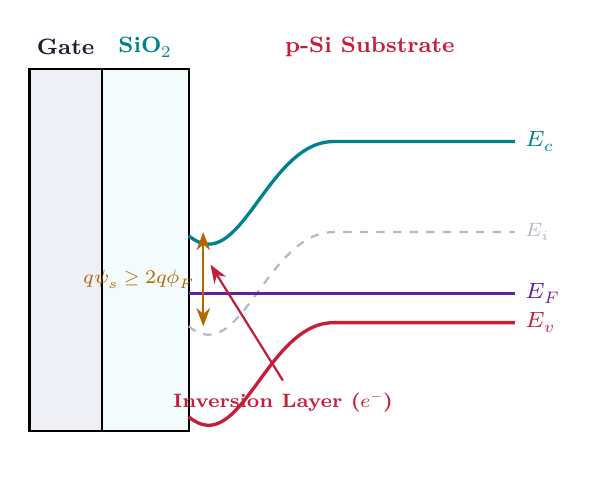
\begin{tikzpicture}[scale=0.92]
  % Regions: Metal | Oxide | Silicon
  \draw[thick, fill=hdrgray] (-3.2, -1.5) rectangle (-2.2, 3.5);
  \node[font=\footnotesize\bfseries\color{mydark}] at (-2.7, 3.8) {Gate};

  \draw[thick, fill=hdrteal!30] (-2.2, -1.5) rectangle (-1.0, 3.5);
  \node[font=\footnotesize\bfseries\color{myteal}] at (-1.6, 3.8) {$\text{SiO}_2$};

  \node[font=\footnotesize\bfseries\color{myred}] at (1.5, 3.8) {p-Si Substrate};

  % Energy bands in Silicon
  % Ec bending down
  \draw[very thick, color=myteal] (-1.0, 1.2) to[out=-40, in=180] (1.0, 2.5) -- (3.5, 2.5) node[right, font=\footnotesize\bfseries] {$E_c$};
  % Ev bending down
  \draw[very thick, color=myred] (-1.0, -1.3) to[out=-40, in=180] (1.0, 0.0) -- (3.5, 0.0) node[right, font=\footnotesize\bfseries] {$E_v$};
  % Ei dashed bending down
  \draw[dashed, thick, color=mgframe] (-1.0, -0.05) to[out=-40, in=180] (1.0, 1.25) -- (3.5, 1.25) node[right, font=\scriptsize] {$E_i$};

  % EF flat horizontal
  \draw[very thick, color=mypurple] (-1.0, 0.4) -- (3.5, 0.4) node[right, font=\footnotesize\bfseries] {$E_F$};

  % Potential indicators
  \draw[Stealth-Stealth, thick, color=myamber] (-0.8, -0.05) -- (-0.8, 1.25) node[midway, left, font=\scriptsize\bfseries] {$q\psi_s \ge 2q\phi_F$};
  \node[font=\scriptsize\bfseries\color{myred}] at (0.3, -1.1) {Inversion Layer ($e^-$)};
  \draw[-Stealth, thick, color=myred] (0.3, -0.8) -- (-0.7, 0.8);
\end{tikzpicture}
\end{tcolorbox}

\subsection{Threshold Voltage Derivation}
At the onset of strong inversion ($\psi_s = 2\phi_F$), the depletion region reaches its maximum width $W_{\text{max}}$:
\begin{equation}
  W_{\text{max}} = \sqrt{\frac{4 \epsilon_s \phi_F}{q N_A}}
\end{equation}
Beyond this point, any further increase in gate voltage is shielded by the exponentially growing inversion electron charge, locking the depletion width at $W_{\text{max}}$. The maximum depletion charge per unit area is:
\begin{equation}
  Q_{d,\text{max}} = -q N_A W_{\text{max}} = -\sqrt{4 q \epsilon_s N_A \phi_F}
\end{equation}

By voltage loop across the MOS structure, the applied gate threshold voltage $V_T$ is:
\begin{equation}
  V_T = V_{FB} + V_{ox} + \psi_s = V_{FB} - \frac{Q_{d,\text{max}}}{C_{ox}} + 2\phi_F
\end{equation}

\begin{tcolorbox}[formulabox, title={\textbf{Threshold Voltage and Body Effect Equations}}]
\begin{equation}
  V_{T0} = V_{FB} + 2\phi_F + \frac{\sqrt{4 q \epsilon_s N_A \phi_F}}{C_{ox}}
\end{equation}
When a reverse substrate-to-source body bias ($V_{SB} > 0$) is applied:
\begin{equation}
  V_T = V_{T0} + \gamma \left(\sqrt{2\phi_F + V_{SB}} - \sqrt{2\phi_F}\right)
\end{equation}
where $\gamma$ is the \textbf{body effect coefficient}:
\begin{equation}
  \gamma = \frac{\sqrt{2 q \epsilon_s N_A}}{C_{ox}} \quad (\text{V}^{1/2})
\end{equation}
\end{tcolorbox}

% ===============================================================================
\section{C-V Characteristics of the MOS Capacitor}
% ===============================================================================

The capacitance of an MOS capacitor is defined as $C = dQ_G / dV_G$. The total capacitance is the series combination of the fixed oxide capacitance $C_{ox}$ and the semiconductor surface capacitance $C_s$:

\begin{equation}
  C = \frac{C_{ox} C_s}{C_{ox} + C_s}
\end{equation}

\par\vspace{6pt}\noindent
\begingroup
\setlength{\tabcolsep}{5pt}
\setlength{\extrarowheight}{3pt}
\renewcommand{\arraystretch}{1.35}
\begin{tabularx}{\linewidth}{|B{2.8cm}|Y|Y|}
\hline
\multicolumn{1}{|c|}{\textbf{Bias Regime}} & \multicolumn{1}{c|}{\textbf{Low-Frequency (LF) Capacitance}} & \multicolumn{1}{c|}{\textbf{High-Frequency (HF) Capacitance}} \\
\hline
Accumulation ($V_G < V_{FB}$) & $C = C_{ox}$ \newline Majority holes accumulate immediately at interface ($C_s \to \infty$). & $C = C_{ox}$ \newline Majority holes respond rapidly up to multi-GHz frequencies. \\
\hline
Depletion ($V_{FB} < V_G < V_T$) & $C = \frac{C_{ox} C_{\text{dep}}}{C_{ox} + C_{\text{dep}}} < C_{ox}$ \newline Decreases monotonically as depletion layer widens ($W \propto \sqrt{\psi_s}$). & $C = \frac{C_{ox} C_{\text{dep}}}{C_{ox} + C_{\text{dep}}} < C_{ox}$ \newline Depletion layer capacitance dominates identically for LF and HF. \\
\hline
Strong Inversion ($V_G \ge V_T$) & $C = C_{ox}$ \newline Thermal generation-recombination ($1\text{--}100\,\text{Hz}$) keeps pace with slow AC signal; inversion charge $Q_n$ modulates. & $C = C_{\text{min}} = \frac{C_{ox} C_{\text{dep,max}}}{C_{ox} + C_{\text{dep,max}}}$ \newline Minority carriers cannot respond ($f \ge 100\,\text{kHz}$); depletion layer stays locked at $W_{\text{max}}$. \\
\hline
Deep Depletion (Fast Ramp) & Not observed under slow quasi-static sweeps. & $C$ continues to decrease below $C_{\text{min}}$ because inversion layer has no time to generate; $W > W_{\text{max}}$. \\
\hline
\end{tabularx}
\endgroup

\begin{tcolorbox}[tikzbox, title={MOS Capacitor Low-Frequency and High-Frequency C-V Curves}]
\centering
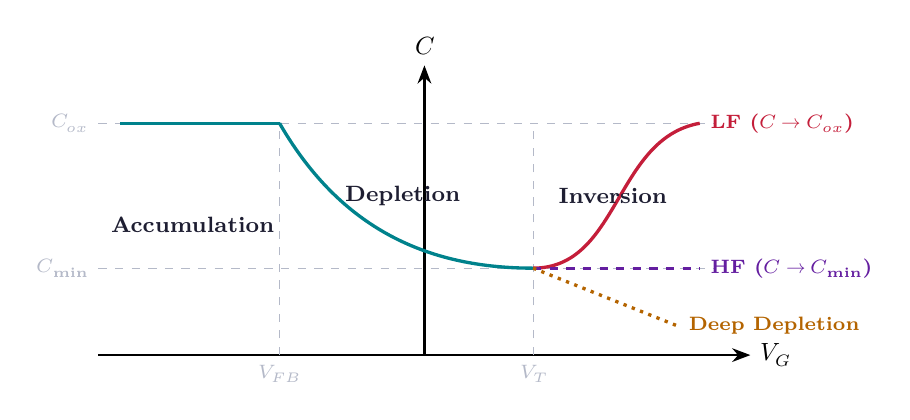
\begin{tikzpicture}[scale=0.92]
  \draw[-Stealth, thick] (-4.5, 0) -- (4.5, 0) node[right, font=\small] {$V_G$};
  \draw[-Stealth, thick] (0, 0) -- (0, 4.0) node[above, font=\small] {$C$};

  % Coordinates
  \coordinate (Cox) at (-4.0, 3.2);
  \coordinate (VFB) at (-2.0, 0);
  \coordinate (VT) at (1.5, 0);

  % Ticks
  \draw[dashed, color=mgframe] (-2.0, 0) node[below, font=\scriptsize] {$V_{FB}$} -- (-2.0, 3.2);
  \draw[dashed, color=mgframe] (1.5, 0) node[below, font=\scriptsize] {$V_T$} -- (1.5, 3.2);
  \draw[dashed, color=mgframe] (-4.5, 3.2) node[left, font=\scriptsize\bfseries\color{mydark}] {$C_{ox}$} -- (4.0, 3.2);
  \draw[dashed, color=mgframe] (-4.5, 1.2) node[left, font=\scriptsize\bfseries\color{mydark}] {$C_{\text{min}}$} -- (4.0, 1.2);

  % Accumulation Flat region
  \draw[very thick, color=myteal] (-4.2, 3.2) -- (-2.0, 3.2);

  % Depletion drop
  \draw[very thick, color=myteal] (-2.0, 3.2) to[out=-60, in=180] (1.5, 1.2);

  % Low-frequency recovery to Cox
  \draw[very thick, color=myred] (1.5, 1.2) to[out=0, in=-170] (3.8, 3.2) node[right, font=\scriptsize\bfseries\color{myred}] {LF ($C \to C_{ox}$)};

  % High-frequency flat at Cmin
  \draw[very thick, dashed, color=mypurple] (1.5, 1.2) -- (3.8, 1.2) node[right, font=\scriptsize\bfseries\color{mypurple}] {HF ($C \to C_{\text{min}}$)};

  % Deep depletion
  \draw[very thick, dotted, color=myamber] (1.5, 1.2) -- (3.5, 0.4) node[right, font=\scriptsize\bfseries\color{myamber}] {Deep Depletion};

  \node[font=\footnotesize\bfseries\color{mydark}] at (-3.2, 1.8) {Accumulation};
  \node[font=\footnotesize\bfseries\color{mydark}] at (-0.3, 2.2) {Depletion};
  \node[font=\footnotesize\bfseries\color{mydark}] at (2.6, 2.2) {Inversion};
\end{tikzpicture}
\end{tcolorbox}

% ===============================================================================
\section{MOSFET Operation and I-V Characteristics}
% ===============================================================================

The MOSFET is a four-terminal, voltage-controlled majority carrier field-effect transistor. By utilizing heavily doped Source and Drain regions that act as reservoirs of mobile electrons, the inversion channel can be modulated instantly, bypassing the slow thermal generation limit of the MOS capacitor.

\subsection{Operating Regimes of an n-Channel Enhancement MOSFET}
\begin{enumerate}[label=\arabic*., leftmargin=*]
  \item \textbf{Cut-off Region ($V_{GS} < V_T$):}
  No continuous inversion channel connects the source and drain. The drain-to-source path comprises two back-to-back p-n junctions ($n^+\text{--}p\text{--}n^+$). Ideal current $I_D = 0$. (In practice, subthreshold diffusion current flows: $I_D \propto \exp\left(\frac{V_{GS} - V_T}{n V_T}\right)$).

  \item \textbf{Linear / Triode Region ($V_{GS} \ge V_T$ and $V_{DS} < V_{GS} - V_T$):}
  An unbroken conducting channel exists from source to drain. The inversion charge density decreases smoothly from source ($Q_n(0) = -C_{ox}(V_{GS} - V_T)$) to drain ($Q_n(L) = -C_{ox}(V_{GS} - V_T - V_{DS})$). Integrating drift current:
  \begin{equation}
    I_D = \mu_n C_{ox} \frac{W}{L} \left[ (V_{GS} - V_T) V_{DS} - \frac{1}{2} V_{DS}^2 \right]
  \end{equation}
  For small $V_{DS} \ll 2(V_{GS} - V_T)$, the $V_{DS}^2$ term is negligible, and the MOSFET acts as a linear \textbf{voltage-controlled resistor}:
  \begin{equation}
    r_{DS} = \left(\frac{\partial I_D}{\partial V_{DS}}\right)^{-1} = \frac{1}{\mu_n C_{ox} \frac{W}{L} (V_{GS} - V_T)}
  \end{equation}

  \item \textbf{Pinch-Off and Saturation Region ($V_{GS} \ge V_T$ and $V_{DS} \ge V_{DS,\text{sat}} = V_{GS} - V_T$):}
  When $V_{DS}$ reaches the \textbf{saturation voltage} $V_{DS,\text{sat}} = V_{GS} - V_T$, the inversion layer charge at the drain end drops to zero ($Q_n(L) = 0$). This point is called \textbf{pinch-off}.
  \begin{itemize}
    \item Any further increase in $V_{DS}$ cannot increase the voltage drop across the remaining channel; the excess voltage $(V_{DS} - V_{DS,\text{sat}})$ is dropped across the high-field drain depletion region.
    \item Electrons reaching the pinch-off point are swept across the depletion space by the high electric field into the drain.
    \item Substituting $V_{DS} = V_{GS} - V_T$ yields the square-law saturation equation:
  \end{itemize}
  \begin{equation}
    I_{D,\text{sat}} = \frac{1}{2} \mu_n C_{ox} \frac{W}{L} (V_{GS} - V_T)^2
  \end{equation}
\end{enumerate}

\subsection{Channel Length Modulation (CLM)}
In the saturation region, as $V_{DS}$ increases past $V_{DS,\text{sat}}$, the pinch-off point migrates slightly toward the source. The effective channel length becomes $L_{\text{eff}} = L - \Delta L$. Because $I_D \propto 1/L_{\text{eff}}$, current rises slightly with $V_{DS}$:

\begin{tcolorbox}[formulabox, title={\textbf{MOSFET Saturation Current with Channel Length Modulation}}]
\begin{equation}
  I_D = \frac{1}{2} \mu_n C_{ox} \frac{W}{L} (V_{GS} - V_T)^2 \left( 1 + \lambda V_{DS} \right)
\end{equation}
where $\lambda = \frac{1}{V_A}$ is the \textbf{channel length modulation parameter} ($\text{V}^{-1}$), and $V_A$ is the MOSFET Early voltage ($V_A \propto L$).
\end{tcolorbox}

% ===============================================================================
\section{Small Signal Models of the MOS Transistor}
% ===============================================================================

\subsection{Low-Frequency Small-Signal Model Parameters}
Around a DC operating point ($V_{GS}, V_{DS}, V_{BS}, I_D$) in the saturation region:

\begin{enumerate}[label=\arabic*., leftmargin=*]
  \item \textbf{Transconductance ($g_m$):} Relates drain current variation to gate-to-source voltage changes:
  \begin{tcolorbox}[formulabox, title={\textbf{Three Equivalent Formulas for Transconductance $g_m$}}]
  \begin{equation}
    g_m = \left.\frac{\partial I_D}{\partial V_{GS}}\right|_{V_{DS}} = \mu_n C_{ox} \frac{W}{L} (V_{GS} - V_T) = \sqrt{2 \mu_n C_{ox} \frac{W}{L} I_D} = \frac{2 I_D}{V_{GS} - V_T}
  \end{equation}
  \end{tcolorbox}

  \item \textbf{Body Transconductance ($g_{mb}$):} Accounts for substrate voltage modulation via the body effect:
  \begin{equation}
    g_{mb} = \left.\frac{\partial I_D}{\partial V_{BS}}\right| = \left(\frac{\partial I_D}{\partial V_T}\right) \left(-\frac{\partial V_T}{\partial V_{SB}}\right) = \frac{\gamma}{2\sqrt{2\phi_F + V_{SB}}} g_m = \eta g_m
  \end{equation}
  where $\eta = \frac{g_{mb}}{g_m} \approx 0.1\text{--}0.25$.

  \item \textbf{Output Resistance ($r_o$):} Arises from channel length modulation:
  \begin{equation}
    r_o = \left.\left(\frac{\partial I_D}{\partial V_{DS}}\right)^{-1}\right|_{V_{GS}} = \frac{1}{\lambda I_D} = \frac{V_A}{I_D}
  \end{equation}
\end{enumerate}

\begin{tcolorbox}[tikzbox, title={Complete Small-Signal Equivalent Circuit of MOSFET (High-Frequency)}]
\centering
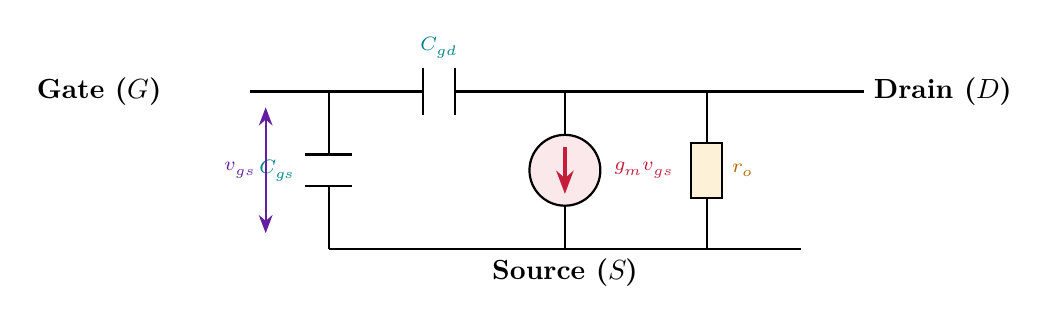
\begin{tikzpicture}[scale=1.0]
  % Gate terminal
  \node[left, font=\normalsize\bfseries] at (-4.0, 2.0) {Gate ($G$)};
  \draw[thick] (-3.0, 2.0) -- (-2.0, 2.0);

  % Source terminal (bottom ground line)
  \draw[thick] (-2.0, 0) -- (4.0, 0);
  \node[below, font=\normalsize\bfseries] at (1.0, 0) {Source ($S$)};

  % Cgs capacitor
  \draw[thick] (-2.0, 2.0) -- (-2.0, 1.2);
  \draw[thick] (-2.3, 1.2) -- (-1.7, 1.2);
  \draw[thick] (-2.3, 0.8) -- (-1.7, 0.8);
  \draw[thick] (-2.0, 0.8) -- (-2.0, 0);
  \node[left, font=\scriptsize\bfseries\color{myteal}] at (-2.3, 1.0) {$C_{gs}$};

  % vgs label
  \draw[Stealth-Stealth, thick, color=mypurple] (-2.8, 1.8) -- (-2.8, 0.2) node[midway, left, font=\scriptsize\bfseries] {$v_{gs}$};

  % Cgd bridging to Drain
  \draw[thick] (-2.0, 2.0) -- (-0.8, 2.0);
  \draw[thick] (-0.8, 2.3) -- (-0.8, 1.7);
  \draw[thick] (-0.4, 2.3) -- (-0.4, 1.7);
  \draw[thick] (-0.4, 2.0) -- (4.0, 2.0);
  \node[above, font=\scriptsize\bfseries\color{myteal}] at (-0.6, 2.3) {$C_{gd}$};

  % Dependent current source gm * vgs
  \draw[thick] (1.0, 2.0) -- (1.0, 1.45);
  \draw[thick, fill=hdrred] (1.0, 1.0) circle (0.45);
  \draw[-Stealth, very thick, color=myred] (1.0, 1.3) -- (1.0, 0.7);
  \node[right, font=\scriptsize\bfseries\color{myred}] at (1.5, 1.0) {$g_m v_{gs}$};
  \draw[thick] (1.0, 0.55) -- (1.0, 0);

  % Output resistor ro
  \draw[thick] (2.8, 2.0) -- (2.8, 1.35);
  \draw[thick, fill=hdramber] (2.6, 0.65) rectangle (3.0, 1.35);
  \node[right, font=\scriptsize\bfseries\color{myamber}] at (3.0, 1.0) {$r_o$};
  \draw[thick] (2.8, 0.65) -- (2.8, 0);

  % Drain terminal
  \draw[thick] (4.0, 2.0) -- (4.8, 2.0);
  \node[right, font=\normalsize\bfseries] at (4.8, 2.0) {Drain ($D$)};
\end{tikzpicture}
\end{tcolorbox}

\subsection{Unity-Gain Cut-Off Frequency (\texorpdfstring{$f_T$}{fT})}
The transition frequency $f_T$ is the frequency at which the short-circuit AC current gain of the common-source MOSFET drops to unity ($|i_d / i_g| = 1$):

\begin{tcolorbox}[formulabox, title={\textbf{Unity-Gain Cut-Off Frequency}}]
\begin{equation}
  f_T = \frac{g_m}{2\pi (C_{gs} + C_{gd})} \approx \frac{\mu_n C_{ox} \frac{W}{L} (V_{GS} - V_T)}{2\pi \left(\frac{2}{3} W L C_{ox}\right)} = \frac{3 \mu_n (V_{GS} - V_T)}{4\pi L^2}
\end{equation}
\textbf{Scaling Law:} $f_T \propto 1/L^2$. Reducing physical channel length $L$ yields a quadratic increase in operating speed and device bandwidth.
\end{tcolorbox}

\newpage
% ===============================================================================
% MANDATORY QUICK REVISION PAGE
% ===============================================================================
\begin{center}
  {\large\bfseries\color{myred} Quick Revision --- Module 3}\\[3pt]
  {\small\color{mydark} MOSFET Physics, C-V \& Small Signal Models $|$ EC301}
\end{center}
\noindent{\color{myred}\rule{\linewidth}{1.2pt}}
\vspace{4pt}

\begin{tcolorbox}[formulabox, title={\textbf{Key Formulas and Metrics at a Glance}}]
\renewcommand{\arraystretch}{1.35}
\begin{tabularx}{\linewidth}{B{5.0cm} X}
Oxide Capacitance per Area & $C_{ox} = \frac{\epsilon_{ox}}{t_{ox}}$ \\[4pt]
Flat-Band Voltage ($V_{FB}$) & $V_{FB} = \Phi_{ms} - \frac{Q_{ox}}{C_{ox}}$ \\[4pt]
Threshold Voltage ($V_{T0}$) & $V_{T0} = V_{FB} + 2\phi_F + \frac{\sqrt{4q\epsilon_s N_A \phi_F}}{C_{ox}}$ \\[4pt]
Body Effect Threshold Shift & $V_T = V_{T0} + \gamma \left(\sqrt{2\phi_F + V_{SB}} - \sqrt{2\phi_F}\right)$ \\[4pt]
Linear Region Drain Current & $I_D = \mu_n C_{ox} \frac{W}{L} \left[(V_{GS}-V_T)V_{DS} - \frac{1}{2}V_{DS}^2\right]$ \\[4pt]
Saturation Drain Current & $I_{D,\text{sat}} = \frac{1}{2}\mu_n C_{ox}\frac{W}{L}(V_{GS}-V_T)^2(1+\lambda V_{DS})$ \\[4pt]
Transconductance ($g_m$) & $g_m = \mu_n C_{ox}\frac{W}{L}(V_{GS}-V_T) = \sqrt{2\mu_n C_{ox}\frac{W}{L}I_D}$ \\[4pt]
Output Resistance ($r_o$) & $r_o = \frac{1}{\lambda I_D} = \frac{V_A}{I_D}$ \\[4pt]
Unity-Gain Frequency ($f_T$) & $f_T \approx \frac{g_m}{2\pi C_{gs}} \approx \frac{3\mu_n(V_{GS}-V_T)}{4\pi L^2}$ \\[4pt]
Maximum Depletion Width & $W_{\text{max}} = \sqrt{\frac{4\epsilon_s \phi_F}{q N_A}}$ \\[4pt]
\end{tabularx}
\end{tcolorbox}

\begin{tcolorbox}[defbox, title={\textbf{One-Line Definitions}}]
\begin{itemize}[leftmargin=*, itemsep=2pt, topsep=0pt]
  \item \textbf{Flat-Band Voltage ($V_{FB}$):} Gate voltage required to negate work-function differences and oxide charges, making bands flat.
  \item \textbf{Strong Inversion:} State where surface potential $\psi_s \ge 2\phi_F$, creating an electron sheet equal to bulk hole doping.
  \item \textbf{Pinch-Off:} Phenomenon where inversion channel charge at the drain vanishes when $V_{DS} \ge V_{GS} - V_T$.
  \item \textbf{Body Effect:} Increase in threshold voltage caused by applying a reverse bias between source and body substrate.
  \item \textbf{Channel Length Modulation:} Shortening of the effective channel length under high $V_{DS}$, producing finite output resistance.
  \item \textbf{Transconductance ($g_m$):} Rate of change of drain current with respect to gate-source voltage at constant $V_{DS}$.
  \item \textbf{Transition Frequency ($f_T$):} Frequency at which the small-signal short-circuit current gain drops to unity ($0\,\text{dB}$).
\end{itemize}
\end{tcolorbox}

\begin{tcolorbox}[exambox, title={\textbf{Frequently Asked / Viva Questions}}]
\begin{enumerate}[topsep=0pt, label=\textbf{Q\arabic*.}, itemsep=5pt]
  \item \Q{Why does the high-frequency C-V curve of an MOS capacitor remain at $C_{\text{min}}$ in inversion while the low-frequency curve recovers to $C_{ox}$?}
    In an isolated MOS capacitor, minority electrons can only be supplied via thermal generation-recombination across the bandgap, which is slow ($\tau \sim 0.01\text{--}0.1\,\text{s}$). At high frequencies ($f \ge 100\,\text{kHz}$), minority electrons cannot follow the AC signal, so the depletion layer capacitance $C_{\text{dep,max}}$ remains in series with $C_{ox}$, locking total capacitance at $C_{\text{min}}$. At low frequencies ($f \le 100\,\text{Hz}$), minority carriers respond, shielding the silicon bulk and restoring $C = C_{ox}$.
  \item \Q{Why does a MOSFET invert instantaneously while a standalone MOS capacitor takes significant time?}
    A MOSFET has heavily doped $n^+$ Source and Drain regions immediately adjacent to the channel, providing an abundant reservoir of electrons that can flow into the channel within picoseconds, whereas an MOS capacitor must wait for slow thermal EHP generation.
  \item \Q{What is the physical condition for the onset of strong inversion?}
    The surface potential must equal twice the bulk Fermi potential: $\psi_s = 2\phi_F = 2 V_T \ln(N_A / n_i)$. At this potential, the surface electron concentration $n_s = n_i e^{(\psi_s - \phi_F)/V_T}$ equals the substrate acceptor concentration $N_A$.
  \item \Q{Explain the physical mechanism of the Body Effect in a MOSFET.}
    Applying a reverse substrate bias ($V_{SB} > 0$) widens the depletion layer beneath the gate, exposing additional negative acceptor ions ($-q N_A$). The gate voltage must support this additional depletion charge before creating the inversion layer, thereby increasing $V_T$.
  \item \Q{What is Channel Length Modulation (CLM) and what is its effect on amplifier gain?}
    In saturation, high $V_{DS}$ shifts the pinch-off point toward the source, decreasing effective channel length $L_{\text{eff}} = L - \Delta L$. This causes drain current to increase with $V_{DS}$, giving the MOSFET a finite output resistance $r_o = 1/(\lambda I_D)$ and limiting maximum intrinsic voltage gain $A_{v0} = g_m r_o$.
  \item \Q{Compare enhancement-mode and depletion-mode MOSFETs.}
    Enhancement-mode MOSFETs have no physical channel at $V_{GS} = 0$ (normally OFF) and require $V_{GS} > V_T > 0$ to conduct. Depletion-mode MOSFETs have an implanted physical channel at $V_{GS} = 0$ (normally ON) and require a negative gate voltage $V_{GS} < V_T < 0$ to deplete the channel and turn off.
  \item \Q{Why is an n-channel MOSFET faster and smaller than a p-channel MOSFET for the same drive current?}
    Electron mobility in Silicon ($\mu_n \approx 1350\,\text{cm}^2/\text{V}\cdot\text{s}$) is nearly three times higher than hole mobility ($\mu_p \approx 480\,\text{cm}^2/\text{V}\cdot\text{s}$). To achieve equal current ($I_D \propto \mu W/L$), a PMOS device must be designed with roughly $2.5\text{--}3$ times greater width $W$, which increases parasitic capacitance and area.
  \item \Q{How does the unity-gain frequency $f_T$ depend on MOSFET gate length?}
    $f_T \approx \frac{3\mu_n(V_{GS}-V_T)}{4\pi L^2} \propto \frac{1}{L^2}$. It scales inversely with the square of the channel length, which has been the primary technological driving force behind semiconductor feature scaling.
  \item \Q{What is deep depletion in an MOS capacitor?}
    Deep depletion occurs when a rapid positive voltage ramp is applied to the gate so fast that no inversion electrons can generate. The depletion layer expands past $W_{\text{max}}$, and capacitance continues dropping below $C_{\text{min}}$. This state is utilized in CCD image sensors.
  \item \Q{What is the transconductance parameter $k_n'$ and device transconductance parameter $k_n$?}
    Process transconductance parameter $k_n' = \mu_n C_{ox}$ ($\text{A/V}^2$), which depends purely on fabrication technology. Device transconductance parameter $k_n = k_n' (W/L) = \mu_n C_{ox} (W/L)$, which depends on circuit designer sizing.
\end{enumerate}
\end{tcolorbox}

\begin{tcolorbox}[tikzbox, title={Comparison of BJT and MOSFET Device Characteristics}]
\centering
\renewcommand{\arraystretch}{1.45}
\begin{tabularx}{\linewidth}{|B{3.2cm}|Y|Y|}
\hline
\multicolumn{1}{|c|}{\textbf{Parameter}} & \multicolumn{1}{c|}{\textbf{Bipolar Junction Transistor (BJT)}} & \multicolumn{1}{c|}{\textbf{MOSFET}} \\
\hline
Operating Principle & Current-controlled device ($I_C = \beta I_B$) & Voltage-controlled device ($I_D \propto V_{GS}^2$) \\
\hline
Carrier Type & Bipolar (both electrons and holes participate) & Unipolar (majority carriers only in channel) \\
\hline
Input Impedance & Low to moderate ($1\text{--}10\,\text{k}\Omega$ in active mode) & Extremely high ($> 10^{12}\,\Omega$, isolated gate oxide) \\
\hline
Input Current & Continuous DC base current $I_B = I_C / \beta$ & Zero static gate current ($I_G \approx 0$) \\
\hline
Temperature Coefficient & Negative ($\text{NTC}$): prone to thermal runaway & Positive ($\text{PTC}$): thermally self-limiting \\
\hline
Noise Figure & Low $1/f$ flicker noise; higher shot noise & Higher flicker noise ($1/f$ interface states) \\
\hline
Fabrication Density & Moderate; requires isolation wells & Extremely high; self-aligned planar process \\
\hline
Primary Applications & High-speed RF, precision analog, linear power & Digital VLSI, microprocessors, CMOS logic, power \\
\hline
\end{tabularx}
\end{tcolorbox}


% -- Module 4 -----------------------------------------------------------------
\modulestart{4}{Optical Absorption in Semiconductors}

\section{Optical Absorption in Semiconductors}
% ===============================================================================

Optoelectronic devices operate via the conversion of optical energy (photons) into electrical energy (electrons and holes), or vice versa.

\subsection{Fundamental Optical Absorption Process}
When incident photons strike a semiconductor:
\begin{itemize}[leftmargin=*, itemsep=3pt]
  \item If photon energy is less than the bandgap ($h\nu < E_g$), the semiconductor cannot absorb the photon; the material is transparent to that wavelength.
  \item If photon energy equals or exceeds the bandgap ($h\nu \ge E_g$), the photon is absorbed, elevating a valence electron into the conduction band and creating an \textbf{electron-hole pair (EHP)}.
  \item The \textbf{cut-off wavelength} ($\lambda_c$) above which no band-to-band optical absorption can occur is:
  \begin{equation}
    \lambda_c = \frac{hc}{E_g} = \frac{1.24}{E_g\,(\text{eV})}\,\mu\text{m}
  \end{equation}
  For Silicon ($E_g = 1.12\,\text{eV}$), $\lambda_c \approx 1.11\,\mu\text{m}$ (near infrared). For GaAs ($E_g = 1.42\,\text{eV}$), $\lambda_c \approx 0.87\,\mu\text{m}$.
\end{itemize}

\subsection{Absorption Coefficient and Beer-Lambert's Law}
The attenuation of optical intensity $I(x)$ as light propagates through a distance $x$ within a semiconductor is described by the \textbf{Beer-Lambert Law}:

\begin{tcolorbox}[formulabox, title={\textbf{Beer-Lambert Absorption Law}}]
\begin{equation}
  I(x) = I_0 \exp(-\alpha x)
\end{equation}
where $I_0$ is the incident light intensity (after surface reflection), and $\alpha$ is the \textbf{absorption coefficient} ($\text{cm}^{-1}$). The characteristic \textbf{optical penetration depth} is $\delta = 1/\alpha$. Direct bandgap semiconductors exhibit very steep absorption edges ($\alpha \sim 10^4\text{--}10^5\,\text{cm}^{-1}$, $\delta \sim 0.1\text{--}1\,\mu\text{m}$), whereas indirect bandgap semiconductors require phonon assistance ($\alpha \sim 10^2\text{--}10^3\,\text{cm}^{-1}$, $\delta \sim 10\text{--}100\,\mu\text{m}$).
\end{tcolorbox}

% ===============================================================================
\section{Photovoltaic Effects and Solar Cells}
% ===============================================================================

A \textbf{solar cell} is an un-biased, large-area p-n junction that converts optical solar radiation directly into electrical power via the \textbf{photovoltaic effect}.

\subsection{Physical Working Principle}
\begin{enumerate}[label=\arabic*., leftmargin=*]
  \item Photons with $h\nu \ge E_g$ penetrate the thin top layer and generate EHPs within and adjacent to the space charge depletion layer.
  \item The high built-in electric field $\vec{\mathcal{E}}$ in the depletion region sweeps photogenerated electrons to the n-side and photogenerated holes to the p-side before they can recombine.
  \item This accumulation of charges establishes a forward photovoltage across the terminals, driving an external load current.
\end{enumerate}

\subsection{Equivalent Circuit and Solar Cell I-V Characteristics}
An ideal solar cell is modeled as an ideal light-generated constant current source $I_L$ in parallel with a forward-biased diode:

\begin{tcolorbox}[formulabox, title={\textbf{Solar Cell Current-Voltage Equation}}]
\begin{equation}
  I = I_L - I_D = I_L - I_0 \left[ \exp\left(\frac{q V}{\eta k T}\right) - 1 \right]
\end{equation}
where $I_L$ is the photogenerated current ($I_L \propto \text{incident optical power}$).
\end{tcolorbox}

\begin{tcolorbox}[tikzbox, title={Solar Cell Equivalent Circuit and Fourth-Quadrant I-V Curve}]
\centering
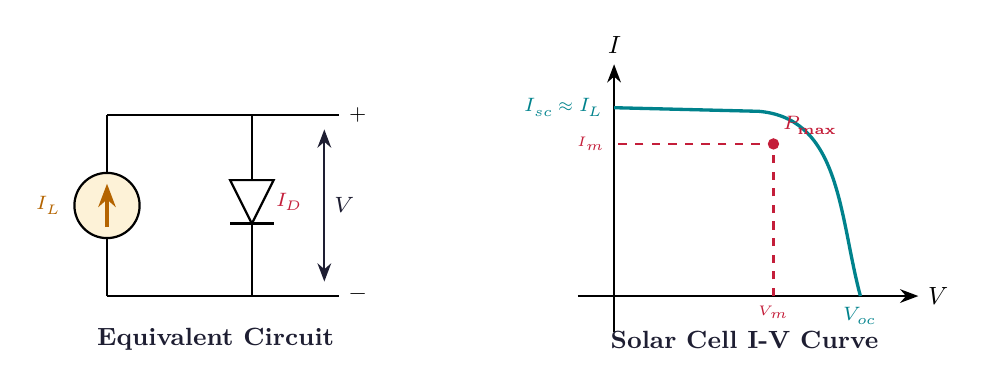
\begin{tikzpicture}[scale=0.92]
  % Equivalent Circuit (Left)
  \begin{scope}[xshift=-4.5cm]
    % Current source IL
    \draw[thick] (0, 0) -- (0, 0.8);
    \draw[thick, fill=hdramber] (0, 1.25) circle (0.45);
    \draw[-Stealth, very thick, color=myamber] (0, 0.95) -- (0, 1.55);
    \node[left, font=\scriptsize\bfseries\color{myamber}] at (-0.5, 1.25) {$I_L$};
    \draw[thick] (0, 1.7) -- (0, 2.5);

    % Diode
    \draw[thick] (0, 2.5) -- (2.0, 2.5) -- (2.0, 1.6);
    \draw[thick] (1.7, 1.6) -- (2.3, 1.6) -- (2.0, 1.0) -- cycle;
    \draw[thick] (1.7, 1.0) -- (2.3, 1.0);
    \draw[thick] (2.0, 1.0) -- (2.0, 0) -- (0, 0);
    \node[right, font=\scriptsize\bfseries\color{myred}] at (2.2, 1.3) {$I_D$};

    % Terminals
    \draw[thick] (2.0, 2.5) -- (3.2, 2.5) node[right, font=\footnotesize\bfseries] {$+$};
    \draw[thick] (2.0, 0) -- (3.2, 0) node[right, font=\footnotesize\bfseries] {$-$};
    \draw[Stealth-Stealth, thick, color=mydark] (3.0, 2.3) -- (3.0, 0.2) node[midway, right, font=\footnotesize\bfseries] {$V$};
    \node[font=\small\bfseries\color{mydark}] at (1.5, -0.6) {Equivalent Circuit};
  \end{scope}

  % I-V Characteristics (Right)
  \begin{scope}[xshift=2.5cm]
    \draw[-Stealth, thick] (-0.5, 0) -- (4.2, 0) node[right, font=\small] {$V$};
    \draw[-Stealth, thick] (0, -0.5) -- (0, 3.2) node[above, font=\small] {$I$};

    % I-V curve
    \draw[very thick, color=myteal] (0, 2.6) node[left, font=\scriptsize\bfseries] {$I_{sc} \approx I_L$} -- (2.0, 2.55) to[out=-5, in=105] (3.4, 0) node[below, font=\scriptsize\bfseries] {$V_{oc}$};

    % Maximum Power Rectangle
    \draw[dashed, thick, color=myred] (2.2, 0) -- (2.2, 2.1) -- (0, 2.1);
    \node[below, font=\tiny\bfseries\color{myred}] at (2.2, 0) {$V_m$};
    \node[left, font=\tiny\bfseries\color{myred}] at (0, 2.1) {$I_m$};
    \filldraw[color=myred] (2.2, 2.1) circle (2pt) node[above right, font=\scriptsize\bfseries] {$P_{\text{max}}$};
    \node[font=\small\bfseries\color{mydark}] at (1.8, -0.6) {Solar Cell I-V Curve};
  \end{scope}
\end{tikzpicture}
\end{tcolorbox}

\subsection{Key Solar Cell Figures of Merit}
\begin{itemize}[leftmargin=*, itemsep=3.5pt]
  \item \textbf{Short-Circuit Current ($I_{sc}$):} Current flowing when terminals are shorted ($V = 0$):
  \begin{equation}
    I_{sc} = I_L
  \end{equation}
  \item \textbf{Open-Circuit Voltage ($V_{oc}$):} Voltage when terminals are open ($I = 0$):
  \begin{equation}
    0 = I_L - I_0 \left[ \exp\left(\frac{q V_{oc}}{\eta k T}\right) - 1 \right] \implies V_{oc} = \eta V_T \ln\left(\frac{I_L}{I_0} + 1\right)
  \end{equation}
  \item \textbf{Maximum Power Point ($P_{\text{max}}$):} Occurs at the knee of the curve where the product $V \cdot I$ is maximized:
  \begin{equation}
    P_{\text{max}} = V_m I_m
  \end{equation}
  \item \textbf{Fill Factor ($FF$):} The ratio of maximum usable power to the theoretical maximum product $V_{oc} I_{sc}$:
  \begin{equation}
    FF = \frac{V_m I_m}{V_{oc} I_{sc}} \quad (\text{typically } 0.70\text{--}0.85)
  \end{equation}
  \item \textbf{Power Conversion Efficiency ($\eta$):}
  \begin{equation}
    \eta = \frac{P_{\text{max}}}{P_{\text{in}}} = \frac{V_{oc} I_{sc} FF}{P_{\text{in}}}
  \end{equation}
  where $P_{\text{in}}$ is the incident solar optical power ($100\,\text{mW/cm}^2$ under AM1.5 standard illumination).
\end{itemize}

% ===============================================================================
\section{Photodetectors: Photoconductors, Photodiodes, PIN and APD}
% ===============================================================================

\subsection{Photoconductors}
A photoconductor is a slab of semiconductor with ohmic contacts at both ends. Light absorption creates excess electron-hole pairs ($\Delta n = \Delta p = g_L \tau$), increasing the material's bulk conductivity:

\begin{equation}
  \Delta \sigma = q (\mu_n + \mu_p) \Delta n = q (\mu_n + \mu_p) g_L \tau
\end{equation}

The \textbf{photoconductive gain} ($G$) is the number of charge carriers passing through the external circuit per absorbed photon:
\begin{equation}
  G = \frac{\tau}{t_{\text{transit}}} = \frac{\tau \mu_n \mathcal{E}}{L} = \frac{\tau \mu_n V}{L^2}
\end{equation}
Because electron lifetime $\tau$ can be much longer than transit time $t_{\text{transit}}$, an electron can circulate through the device multiple times before recombining, producing $G \gg 1$.

\subsection{P-N Photodiode}
A p-n junction operated under \textbf{reverse bias}:
\begin{itemize}[leftmargin=*, itemsep=3pt]
  \item Reverse bias extends the depletion width and creates a high electric field that sweeps photogenerated carriers out rapidly, generating a drift photocurrent:
  \begin{equation}
    I_{\text{total}} = I_0 \left( e^{-V_R / V_T} - 1 \right) - I_{\text{photo}} \approx - (I_0 + I_{\text{photo}})
  \end{equation}
  \item \textbf{Responsivity ($R$):}
  \begin{equation}
    R = \frac{I_{\text{photo}}}{P_{\text{opt}}} = \frac{\eta_{ext} q}{h\nu} = \frac{\eta_{ext} q \lambda}{hc} \quad (\text{A/W})
  \end{equation}
  where $\eta_{ext}$ is the external quantum efficiency.
\end{itemize}

\subsection{PIN Photodiode}
A PIN photodiode inserts a wide, undoped \textbf{intrinsic ($i$)} semiconductor layer between heavily doped $p^+$ and $n^+$ regions ($p^+\text{--}i\text{--}n^+$).

\begin{itemize}[leftmargin=*, itemsep=3pt]
  \item Even under small reverse bias, the intrinsic layer is completely depleted ($W \approx W_i$).
  \item \textbf{Key Advantages over standard p-n photodiodes}:
    \begin{enumerate}
      \item \textbf{High Quantum Efficiency:} The wide $W_i$ provides a large volume for optical absorption, ensuring that nearly all incident photons are converted into drift carriers rather than slow diffusion carriers.
      \item \textbf{Low Junction Capacitance:} Because $C_j = \frac{\epsilon_s A}{W_i}$ and $W_i$ is large, capacitance is extremely small ($< 1\,\text{pF}$), drastically reducing the $RC$ time constant.
      \item \textbf{High Speed / Bandwidth:} Operating speeds reach $10\text{--}40\,\text{GHz}$, making PIN diodes standard in fiber-optic communications.
    \end{enumerate}
\end{itemize}

\subsection{Avalanche Photodiode (APD)}
The APD is operated under very high reverse bias close to the avalanche breakdown voltage:
\begin{itemize}[leftmargin=*, itemsep=3pt]
  \item Photo-generated electrons entering the high-field multiplication depletion region acquire sufficient kinetic energy to cause \textbf{impact ionization}, knocking valence electrons into the conduction band.
  \item This secondary carrier multiplication yields an internal current gain $M$:
  \begin{equation}
    M = \frac{I_{\text{out}}}{I_{\text{photo}}} \approx \frac{1}{1 - (V_R / V_{BR})^n} \quad (M \sim 10\text{--}1000)
  \end{equation}
  \item APDs provide superior optical sensitivity for detecting ultra-weak light signals, but introduce avalanche excess noise.
\end{itemize}

\subsection{Phototransistor}
A phototransistor is a BJT whose reverse-biased collector-base junction is exposed to light. Photogenerated base current $I_{\text{photo}}$ acts as base drive, which is multiplied by the transistor current gain:
\begin{equation}
  I_C = (\beta + 1) I_{\text{photo}}
\end{equation}
It provides high optical sensitivity without external amplifiers, but has lower switching speed than PIN photodiodes due to base charge storage.

% ===============================================================================
\section{Light Emitting Diodes and Semiconductor Lasers}
% ===============================================================================

\subsection{Light Emitting Diode (LED)}
An LED is a heavily doped, forward-biased \textbf{direct bandgap} p-n junction (e.g., $\text{GaAs}, \text{GaN}, \text{InGaN}$).
\begin{itemize}[leftmargin=*, itemsep=3pt]
  \item Forward bias injects minority electrons into the p-side and minority holes into the n-side.
  \item Carriers undergo \textbf{spontaneous radiative recombination}, releasing energy as photons:
  \begin{equation}
    \lambda \approx \frac{hc}{E_g} = \frac{1.24}{E_g\,(\text{eV})}\,\mu\text{m}
  \end{equation}
  \item Emits \textbf{incoherent}, non-directional light across a spectral bandwidth $\Delta \lambda \approx 20\text{--}50\,\text{nm}$.
\end{itemize}

\subsection{Semiconductor Laser Diode}
A laser diode produces \textbf{coherent, monochromatic, and highly directional} optical radiation.

\begin{enumerate}[label=\arabic*., leftmargin=*]
  \item \textbf{Three Radiation Processes:}
    \begin{itemize}
      \item \textbf{Stimulated Absorption:} An incoming photon ($h\nu \approx E_g$) is absorbed, exciting an electron from VB to CB.
      \item \textbf{Spontaneous Emission:} An electron drops spontaneously to the VB, emitting an incoherent photon of random phase and direction.
      \item \textbf{Stimulated Emission:} An incident photon stimulates an excited electron in the CB to drop to the VB, emitting a second photon having the \textbf{exact same energy, phase, polarization, and direction} as the stimulating photon.
    \end{itemize}

  \item \textbf{Population Inversion (Bernard-Duraffourg Condition):}
  To achieve net optical gain (stimulated emission exceeding stimulated absorption), the upper CB states must be more populated than lower VB states. This requires heavy forward current injection such that the separation of quasi-Fermi levels exceeds the photon energy:
  \begin{equation}
    E_g < h\nu < E_{Fn} - E_{Fp}
  \end{equation}

  \item \textbf{Optical Cavity (Fabry-Perot Resonator):}
  Cleaved, polished semiconductor crystal facets at both ends act as partially reflecting mirrors, creating an optical feedback cavity that sustains oscillation above the \textbf{threshold current} $I_{th}$.
\end{enumerate}

% ===============================================================================
\section{Integrated Circuit Fabrication Technologies}
% ===============================================================================

Modern Silicon integrated circuits are manufactured on high-purity single-crystal Silicon wafers using sequential planar processing steps:

\subsection{Overview of Unit Fabrication Steps}
\par\vspace{6pt}\noindent
\begingroup
\setlength{\tabcolsep}{5pt}
\setlength{\extrarowheight}{3pt}
\renewcommand{\arraystretch}{1.35}
\begin{tabularx}{\linewidth}{|B{3.2cm}|Y|Y|}
\hline
\multicolumn{1}{|c|}{\textbf{Process Step}} & \multicolumn{1}{c|}{\textbf{Chemical / Physical Principle}} & \multicolumn{1}{c|}{\textbf{Role in IC Manufacturing}} \\
\hline
Thermal Oxidation & $\text{Si} + \text{O}_2 \to \text{SiO}_2$ (Dry) \newline $\text{Si} + 2\text{H}_2\text{O} \to \text{SiO}_2 + 2\text{H}_2$ (Wet) & Creates gate dielectric ($\text{SiO}_2$), diffusion barrier masks, and surface passivation. \\
\hline
Photolithography & Optical UV exposure of photoresist polymer through a photomask followed by chemical development. & Transfers micro/nanometer geometric layout patterns onto wafer layers. \\
\hline
Etching & Chemical dissolution (Wet) or plasma/reactive ion bombardment (Dry RIE). & Selectively removes unmasked oxide, polysilicon, or metal layers with high vertical fidelity. \\
\hline
Thermal Diffusion & High-temperature ($900\text{--}1150^\circ\text{C}$) thermal dopant transport into silicon. & Forms wells and junction depths; isotropic lateral diffusion occurs. \\
\hline
Ion Implantation & High-energy electrostatic acceleration ($10\text{--}400\,\text{keV}$) of dopant ions into silicon lattice. & Forms shallow source/drain junctions, threshold voltage adjustments; highly precise dosage. \\
\hline
Chemical Vapor Deposition (CVD) & Gas-phase precursor chemical reaction at wafer surface (LPCVD, PECVD). & Deposits thin dielectric films ($\text{Si}_3\text{N}_4, \text{SiO}_2$) and polycrystalline silicon gates. \\
\hline
Sputtering (PVD) & High-energy Argon ion bombardment of metal target dislodging atoms onto wafer. & Deposits metal interconnect layers (Aluminum, Copper, Titanium). \\
\hline
\end{tabularx}
\endgroup

\subsection{Photolithography Step-by-Step Sequence}
Photolithography is the repetitive master patterning engine of planar processing:
\begin{align*}
  \text{Wafer Clean} &\to \text{Barrier Oxide Growth} \to \text{Photoresist Coating} \to \text{Soft Bake} \\
  &\to \text{Mask Align \& UV Exposure} \to \text{Development} \\
  &\to \text{Hard Bake} \to \text{Chemical / Plasma Etch} \to \text{Photoresist Stripping}
\end{align*}

\begin{itemize}[leftmargin=*, itemsep=3pt]
  \item \textbf{Positive Photoresist:} Exposed regions become soluble in developer solution and wash away. Final pattern matches mask opaque features.
  \item \textbf{Negative Photoresist:} Exposed regions cross-link and become insoluble; unexposed regions wash away.
\end{itemize}

\subsection{Twin-Tub CMOS Process Flow}
The \textbf{twin-tub CMOS process} fabricates both n-channel (NMOS) and p-channel (PMOS) transistors on a single common substrate by creating separate, optimized n-well and p-well tubs:

\begin{enumerate}[label=\arabic*., leftmargin=*]
  \item \textbf{Substrate Preparation:} Start with a high-resistivity $p^-$ (or $n^-$) epitaxial silicon wafer.
  \item \textbf{Tub Formation (Twin-Well):} Implantation of Phosphorus ions to form the n-well (for PMOS) and Boron ions to form the p-well (for NMOS), followed by a high-temperature drive-in diffusion.
  \item \textbf{Device Isolation (LOCOS or STI):} Shallow Trench Isolation (STI) etched and filled with $\text{SiO}_2$ to isolate adjacent transistor active areas and suppress latch-up.
  \item \textbf{Threshold Voltage ($V_T$) Adjustment:} Shallow Boron/Phosphorus channel implants to tune NMOS and PMOS threshold voltages.
  \item \textbf{Gate Oxide and Polysilicon Gate:} Grow ultra-thin gate oxide ($t_{ox} \sim 1\text{--}2\,\text{nm}$) followed by LPCVD polysilicon deposition, photolithography, and anisotropic dry etching of gates.
  \item \textbf{Self-Aligned Source/Drain Implantation:}
    \begin{itemize}
      \item $n^+$ Arsenic/Phosphorus implant into p-well using polysilicon gate as mask (forms NMOS source/drain).
      \item $p^+$ Boron implant into n-well using gate as mask (forms PMOS source/drain).
    \end{itemize}
  \item \textbf{Interlayer Dielectric (ILD) and Contact Holes:} Deposit CVD oxide, pattern contact windows via RIE.
  \item \textbf{Metallization and Passivation:} Sputter Aluminum/Copper interconnects, pattern metal lines, and deposit protective $\text{Si}_3\text{N}_4$ passivation overcoat.
\end{enumerate}

\begin{tcolorbox}[tikzbox, title={Cross-Section of Completed Twin-Tub CMOS Inverter}]
\centering
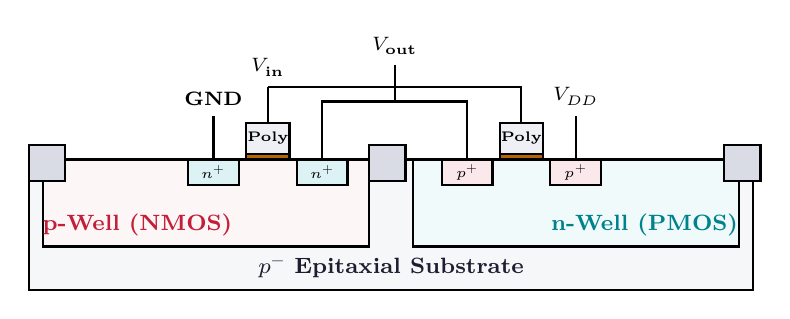
\begin{tikzpicture}[scale=0.92]
  % Substrate
  \draw[thick, fill=mygray] (-5.0, -1.8) rectangle (5.0, 0);
  \node[font=\footnotesize\bfseries\color{mydark}] at (0, -1.5) {$p^-$ Epitaxial Substrate};

  % P-Well (Left)
  \draw[thick, fill=hdrred!40] (-4.8, -1.2) rectangle (-0.3, 0);
  \node[font=\footnotesize\bfseries\color{myred}] at (-3.5, -0.9) {p-Well (NMOS)};

  % N-Well (Right)
  \draw[thick, fill=hdrteal!40] (0.3, -1.2) rectangle (4.8, 0);
  \node[font=\footnotesize\bfseries\color{myteal}] at (3.5, -0.9) {n-Well (PMOS)};

  % STI Isolation Oxide
  \foreach \x in {-5.0, -0.3, 4.6} {
    \draw[thick, fill=mgframe!50] (\x, -0.3) rectangle (\x+0.5, 0.2);
  }

  % NMOS Sources/Drains n+
  \draw[thick, fill=hdrteal] (-2.8, -0.35) rectangle (-2.1, 0) node[midway, font=\tiny\bfseries] {$n^+$};
  \draw[thick, fill=hdrteal] (-1.3, -0.35) rectangle (-0.6, 0) node[midway, font=\tiny\bfseries] {$n^+$};

  % NMOS Gate
  \draw[thick, fill=myamber] (-2.0, 0) rectangle (-1.4, 0.08); % Gate oxide
  \draw[thick, fill=hdrgray] (-2.0, 0.08) rectangle (-1.4, 0.5) node[midway, font=\tiny\bfseries] {Poly};

  % PMOS Sources/Drains p+
  \draw[thick, fill=hdrred] (0.7, -0.35) rectangle (1.4, 0) node[midway, font=\tiny\bfseries] {$p^+$};
  \draw[thick, fill=hdrred] (2.2, -0.35) rectangle (2.9, 0) node[midway, font=\tiny\bfseries] {$p^+$};

  % PMOS Gate
  \draw[thick, fill=myamber] (1.5, 0) rectangle (2.1, 0.08); % Gate oxide
  \draw[thick, fill=hdrgray] (1.5, 0.08) rectangle (2.1, 0.5) node[midway, font=\tiny\bfseries] {Poly};

  % Contact terminals
  \draw[thick] (-1.7, 0.5) -- (-1.7, 1.0) node[above, font=\scriptsize\bfseries] {$V_{\text{in}}$};
  \draw[thick] (1.8, 0.5) -- (1.8, 1.0) -- (-1.7, 1.0);
  \draw[thick] (-0.95, 0) -- (-0.95, 0.8) -- (1.05, 0.8) -- (1.05, 0);
  \draw[thick] (0.05, 0.8) -- (0.05, 1.3) node[above, font=\scriptsize\bfseries] {$V_{\text{out}}$};
  \draw[thick] (-2.45, 0) -- (-2.45, 0.6) node[above, font=\scriptsize\bfseries] {GND};
  \draw[thick] (2.55, 0) -- (2.55, 0.6) node[above, font=\scriptsize\bfseries] {$V_{DD}$};
\end{tikzpicture}
\end{tcolorbox}

\newpage
% ===============================================================================
% MANDATORY QUICK REVISION PAGE
% ===============================================================================
\begin{center}
  {\large\bfseries\color{myred} Quick Revision --- Module 4}\\[3pt]
  {\small\color{mydark} Opto-Electronics \& Integrated Circuit Fabrication $|$ EC301}
\end{center}
\noindent{\color{myred}\rule{\linewidth}{1.2pt}}
\vspace{4pt}

\begin{tcolorbox}[formulabox, title={\textbf{Key Formulas and Metrics at a Glance}}]
\renewcommand{\arraystretch}{1.35}
\begin{tabularx}{\linewidth}{B{5.0cm} X}
Optical Absorption Cut-off & $\lambda_c = \frac{hc}{E_g} = \frac{1.24}{E_g\,(\text{eV})}\,\mu\text{m}$ \\[4pt]
Beer-Lambert Law & $I(x) = I_0 \exp(-\alpha x)$ \\[4pt]
Solar Cell Open-Circuit Voltage & $V_{oc} = \eta V_T \ln\left(\frac{I_L}{I_0} + 1\right)$ \\[4pt]
Solar Cell Fill Factor ($FF$) & $FF = \frac{V_m I_m}{V_{oc} I_{sc}}$ \\[4pt]
Solar Cell Power Efficiency ($\eta$) & $\eta = \frac{V_m I_m}{P_{\text{in}}} = \frac{V_{oc} I_{sc} FF}{P_{\text{in}}}$ \\[4pt]
Photoconductive Gain ($G$) & $G = \frac{\tau}{t_{\text{transit}}} = \frac{\tau \mu V}{L^2}$ \\[4pt]
Photodiode Responsivity ($R$) & $R = \frac{I_{\text{photo}}}{P_{\text{opt}}} = \frac{\eta_{ext} q \lambda}{hc}$ \\[4pt]
Phototransistor Collector Current & $I_C = (\beta + 1) I_{\text{photo}}$ \\[4pt]
Laser Population Inversion & $E_{Fn} - E_{Fp} > h\nu > E_g$ \\[4pt]
APD Multiplication Factor ($M$) & $M = \frac{1}{1 - (V_R / V_{BR})^n}$ \\[4pt]
\end{tabularx}
\end{tcolorbox}

\begin{tcolorbox}[defbox, title={\textbf{One-Line Definitions}}]
\begin{itemize}[leftmargin=*, itemsep=2pt, topsep=0pt]
  \item \textbf{Photovoltaic Effect:} Direct generation of electric potential across a p-n junction caused by absorption of incident photons.
  \item \textbf{Fill Factor ($FF$):} Figure of merit measuring the squareness of a solar cell's fourth-quadrant I-V characteristic.
  \item \textbf{PIN Photodiode:} High-speed, high-efficiency photodetector incorporating a wide intrinsic layer between $p^+$ and $n^+$ regions.
  \item \textbf{Avalanche Photodiode (APD):} Highly sensitive photodetector employing internal carrier multiplication via impact ionization.
  \item \textbf{Population Inversion:} Non-equilibrium condition where the number of electrons in higher energy states exceeds that in lower states.
  \item \textbf{Photolithography:} Microfabrication process transferring photographic geometrical circuit patterns onto a photosensitive polymer resist.
  \item \textbf{Dry Reactive Ion Etching (RIE):} High-resolution anisotropic material removal combining chemical reactivity with directional ion bombardment.
  \item \textbf{Chemical Vapor Deposition (CVD):} Deposition of high-purity solid dielectric or polysilicon thin films from vapor-phase chemical precursors.
\end{itemize}
\end{tcolorbox}

\begin{tcolorbox}[exambox, title={\textbf{Frequently Asked / Viva Questions}}]
\begin{enumerate}[topsep=0pt, label=\textbf{Q\arabic*.}, itemsep=5pt]
  \item \Q{Why does a PIN photodiode possess significantly higher speed and bandwidth than a standard p-n photodiode?}
    In a standard p-n diode, many carriers are generated in neutral regions and must slowly diffuse to the junction ($t_{\text{diff}} \sim \mu\text{s}$). In a PIN diode, the wide intrinsic layer ($W_i$) ensures nearly all photons are absorbed directly within the depletion field, where carriers drift at saturation velocity ($t_{\text{drift}} \sim \text{ps}$). Furthermore, the wide layer significantly reduces junction capacitance ($C_j = \epsilon A / W_i$), decreasing the $RC$ time constant.
  \item \Q{What is the difference between spontaneous emission and stimulated emission?}
    Spontaneous emission occurs randomly without external influence, yielding photons of arbitrary direction and incoherent phase (LED operation). Stimulated emission is triggered by an incoming photon, causing an excited electron to drop and emit a twin photon with identical wavelength, phase, direction, and polarization (Laser operation).
  \item \Q{State the necessary conditions for semiconductor laser operation.}
    \begin{itemize}[leftmargin=*, itemsep=1pt, topsep=2pt]
      \item Population inversion across the bandgap ($E_{Fn} - E_{Fp} > h\nu > E_g$).
      \item Optical cavity feedback (Fabry-Perot resonator) to sustain stimulated emission.
      \item Injection current density exceeding the threshold current density ($J > J_{th}$) where optical gain exceeds cavity losses.
    \end{itemize}
  \item \Q{What is the physical meaning of the Solar Cell Fill Factor ($FF$)?}
    It is the ratio of maximum achievable electric power ($V_m I_m$) to the ideal product ($V_{oc} I_{sc}$). A higher fill factor (approaching $0.85$) represents lower internal series resistance ($R_s \to 0$) and higher shunt resistance ($R_{sh} \to \infty$).
  \item \Q{Why is dry oxidation preferred over wet oxidation for gate oxide growth?}
    Dry oxidation ($\text{Si} + \text{O}_2 \to \text{SiO}_2$) grows very slowly, producing a dense, highly uniform, defect-free oxide film with extremely low interface trap density, which is critical for thin gate dielectrics. Wet oxidation ($\text{Si} + 2\text{H}_2\text{O} \to \text{SiO}_2 + 2\text{H}_2$) is much faster but yields a less dense oxide used for thick masking and field isolation.
  \item \Q{Compare Ion Implantation with Thermal Diffusion for junction doping.}
    Ion implantation allows independent, ultra-precise control over dopant dose and penetration depth, operates at low temperatures, and avoids lateral diffusion under mask edges. Thermal diffusion requires high temperatures ($>1000^\circ\text{C}$), suffers from lateral diffusion, but causes no crystal lattice damage.
  \item \Q{What is the difference between isotropic and anisotropic etching?}
    Isotropic etching (wet chemical) etches equally in all directions, causing significant mask undercut. Anisotropic etching (dry plasma / RIE) etches preferentially in the vertical direction, producing vertical sidewalls essential for sub-micron VLSI layouts.
  \item \Q{Why is the twin-tub CMOS process preferred over single-well CMOS?}
    In single-well CMOS, only one transistor type's well doping can be optimized; the other must use the substrate doping. In the twin-tub process, both n-well and p-well doping profiles and depths can be optimized independently, allowing precise matching of NMOS and PMOS threshold voltages and minimizing latch-up.
  \item \Q{What is photoconductive gain and how can it exceed unity?}
    $G = \tau / t_{\text{transit}}$. When the minority carrier lifetime $\tau$ exceeds the electron transit time $t_{\text{transit}}$, an electron sweeps out of the positive contact while an electron is simultaneously injected from the negative contact to maintain neutrality. The electron circulates through the external circuit multiple times before recombination occurs.
  \item \Q{What is the role of self-alignment in polysilicon gate MOS fabrication?}
    The polysilicon gate electrode acts as an implantation mask for the source and drain implants. This ensures that the edges of the source and drain line up with the edges of the gate, eliminating parasitic gate-to-source and gate-to-drain overlap capacitances.
\end{enumerate}
\end{tcolorbox}

\begin{tcolorbox}[tikzbox, title={Comparison of LED vs. Semiconductor Laser Diode}]
\centering
\renewcommand{\arraystretch}{1.45}
\begin{tabularx}{\linewidth}{|B{3.2cm}|Y|Y|}
\hline
\multicolumn{1}{|c|}{\textbf{Parameter}} & \multicolumn{1}{c|}{\textbf{Light Emitting Diode (LED)}} & \multicolumn{1}{c|}{\textbf{Semiconductor Laser Diode}} \\
\hline
Emission Mechanism & Spontaneous radiative recombination & Stimulated emission with optical cavity feedback \\
\hline
Coherence & Incoherent (random phases) & Highly coherent (identical phase and frequency) \\
\hline
Spectral Width ($\Delta \lambda$) & Wide ($\Delta \lambda \sim 25\text{--}50\,\text{nm}$) & Extremely narrow ($\Delta \lambda \sim 0.1\text{--}2\,\text{nm}$, monochromatic) \\
\hline
Beam Divergence & Wide, non-directional ($\sim 60\text{--}120^\circ$) & Narrow, highly directional ($\sim 5\text{--}15^\circ$) \\
\hline
Threshold Current & No threshold current (emits light at any forward current) & Requires injection current exceeding threshold $I_{th}$ \\
\hline
Modulation Bandwidth & Moderate (tens to hundreds of $\text{MHz}$) & Ultra-high (tens of $\text{GHz}$) \\
\hline
Coupling Efficiency & Low coupling efficiency into optical fibers & High coupling efficiency ($> 80\%$) into single-mode fibers \\
\hline
Applications & Indicators, lighting, short-range plastic fibers & High-speed long-haul optical fiber communications, LiDAR \\
\hline
\end{tabularx}
\end{tcolorbox}


\end{document}
